\documentclass[12pt]{article}
%\usepackage[utf8]{inputenc}
%\documentclass[UTF8]{ctexart}
%\usepackage[UTF8, heading = false, scheme = plain]{ctex}
\usepackage{geometry}
%geometry{a4paper,scale=0.9}
\geometry{a4paper,left=1cm,right=1cm,top=1cm,bottom=2cm}
\usepackage{amsfonts}
\usepackage{color}
\usepackage{url}
%\usepackage{biblatex}
\usepackage{amsmath}
\usepackage{amssymb}
\usepackage{latexsym}
\usepackage[linesnumbered,ruled,lined]{algorithm2e}
\usepackage{cite}
%\addbibresource{ref.bib}
%\bibliography{ref.bib}
\usepackage{caption}
\usepackage{graphicx, subfig}
\usepackage{float}
%\usepackage[fontset=ubuntu]{ctex}
%\usepackage{fontspec}
\usepackage{xeCJK}
%\usepackage[colorlinks,
%anchorcolor=black,
%citecolor=black]{hyperref}
%\setmainfont{SimSun}
\usepackage[section]{placeins}
\usepackage{enumitem}
\usepackage{framed}
\usepackage[framemethod=TikZ]{mdframed}
\usepackage{indentfirst}
\usepackage{setspace}%使用间距宏包
\linespread{1.5}

\title{Embedding 讨论}
\author{leolinuxer}
%\date{June 2020}

\begin{document}
%\setlength{\parindent}{0pt}
\maketitle
\tableofcontents

\part{Embedding 基础概念}
\section{Embedding简介\cite{Embedding_From_Word2Vec_To_Item2Vec}}
\subsection{什么是embedding}
简单来说,embedding就是用一个低维的向量表示一个物体,可以是一个词,或是一个商品,或是一个电影等等。这个embedding向量的性质是能使距离相近的向量对应的物体有相近的含义,比如 Embedding(复仇者联盟)和Embedding(钢铁侠)之间的距离就会很接近,但 Embedding(复仇者联盟)和Embedding(乱世佳人)的距离就会远一些。

除此之外Embedding甚至还具有数学运算的关系,比如Embedding(马德里)-Embedding(西班牙)+Embedding(法国)≈Embedding(巴黎)

言归正传,Embedding能够用低维向量对物体进行编码还能保留其含义的特点非常适合深度学习。在传统机器学习模型构建过程中,我们经常使用one hot encoding对离散特征,特别是id类特征进行编码,但由于one hot encoding的维度等于物体的总数,比如阿里的商品one hot encoding的维度就至少是千万量级的。这样的编码方式对于商品来说是极端稀疏的,甚至用multi hot encoding对用户浏览历史的编码也会是一个非常稀疏的向量。而深度学习的特点以及工程方面的原因使其不利于稀疏特征向量的处理。因此如果能把物体编码为一个低维稠密向量再喂给DNN,自然是一个高效的基本操作。

\subsection{使 embedding 空前流行的 word2vec}
对word的vector表达的研究早已有之,但让embedding方法空前流行,我们还是要归功于google的word2vec。我们简单讲一下word2vec的原理,这对我们之后理解AirBnB对loss function的改进至关重要。

既然我们要训练一个对 word 的语义表达,那么训练样本显然是一个句子的集合。假设其中一个长度为 $T$ 的句子为$w_1, w_2, \cdots, w_T$ 。这时我们假定每个词都跟其相邻的词的关系最密切,换句话说每个词都是由相邻的词决定的(CBOW模型的动机),或者每个词都决定了相邻的词(Skip-gram模型的动机)。如下图,CBOW的输入是 $w_t$ 周边的词,预测的输出是$w_t$,而Skip-gram则反之,经验上讲Skip-gram的效果好一点,所以本文从Skip-gram模型出发讲解模型细节。

\begin{figure}[H]
    \centering
    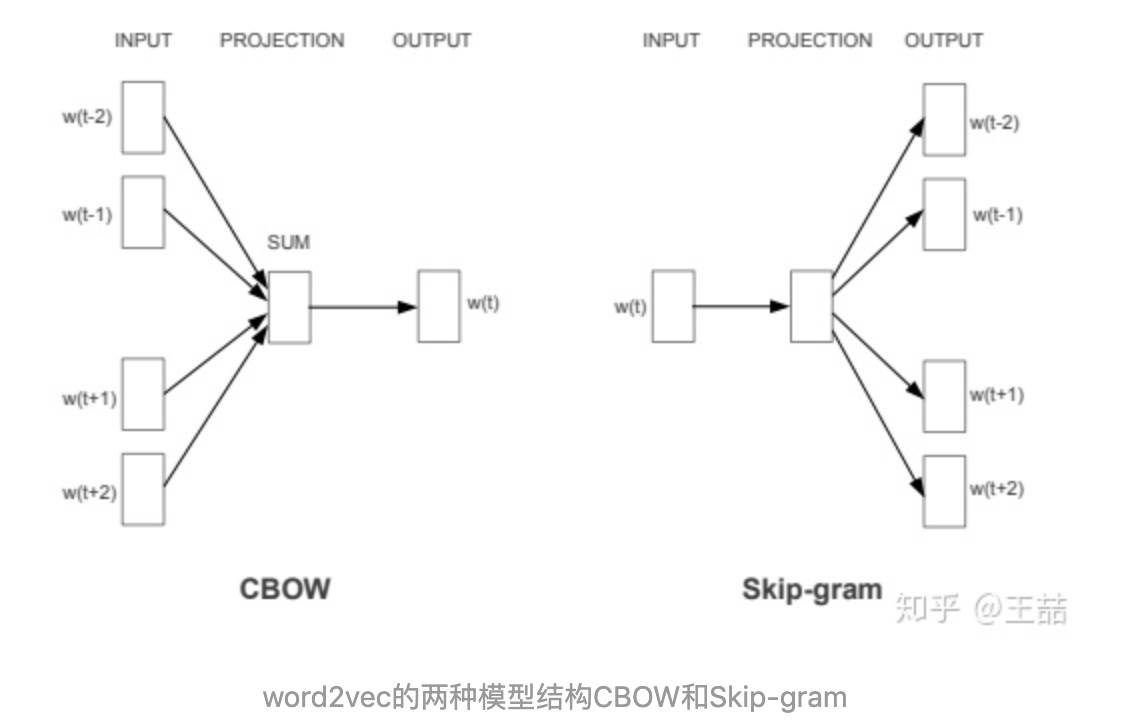
\includegraphics[width=.8\textwidth]{fig/Embedding_Word2vec_Skip-gram_CBOW.png}
\end{figure}

那么为了产生模型的正样本,我们选一个长度为$2c+1$(目标词前后各选$c$个词)的滑动窗口,从句子左边滑倒右边,每滑一次,窗口中的词就形成了我们的一个正样本。

有了训练样本之后我们就可以着手定义优化目标了,既然每个词$w_t$都决定了相邻词 $w_{t+j}$,基于极大似然,我们希望所有样本的条件概率 $p(w_{t+j}|w_t)$ 之积最大,这里我们使用log probability。我们的目标函数有了:
$$
\frac{1}{T} \sum_{t=1}^T\sum_{-c \le j \le c, j \neq 0} \log{p(w_{t+j}|w_t)}
$$

接下来的问题是怎么定义 $p(w_{t+j}|w_t)$ ,作为一个多分类问题,最简单最直接的方法当然是直接用softmax函数,我们又希望用向量$v_w$ 表示每个词 w,用词之间的距离 $v_i^Tv_j$ 表示语义的接近程度,那么我们的条件概率的定义就可以很直观的写出。
$$
P(w_O|w_I) = \frac{\text{exp}({v'}_{w_O}^Tv_{w_I})}{\sum_{w=1}^W\text{exp}({{v'}_{w_O}^Tv_{w_I}})}
$$

看到上面的条件概率公式,很多同学可能会习惯性的忽略一个事实,就是

\textbf{我们用 $w_t$ 去预测 $w_{t+j}$ ,但其实这二者的向量表达并不在一个向量空间内。}

就像上面的条件概率公式写的一样,\textbf{$v'_w$ 和 $v_w$ 分别是词w的输出向量表达和输入向量表达}(??why ??)。那什么是输入向量表达和输出向量表达呢?我们画一个word2vec的神经网络架构图就明白了。
\begin{figure}[H]
    \centering
    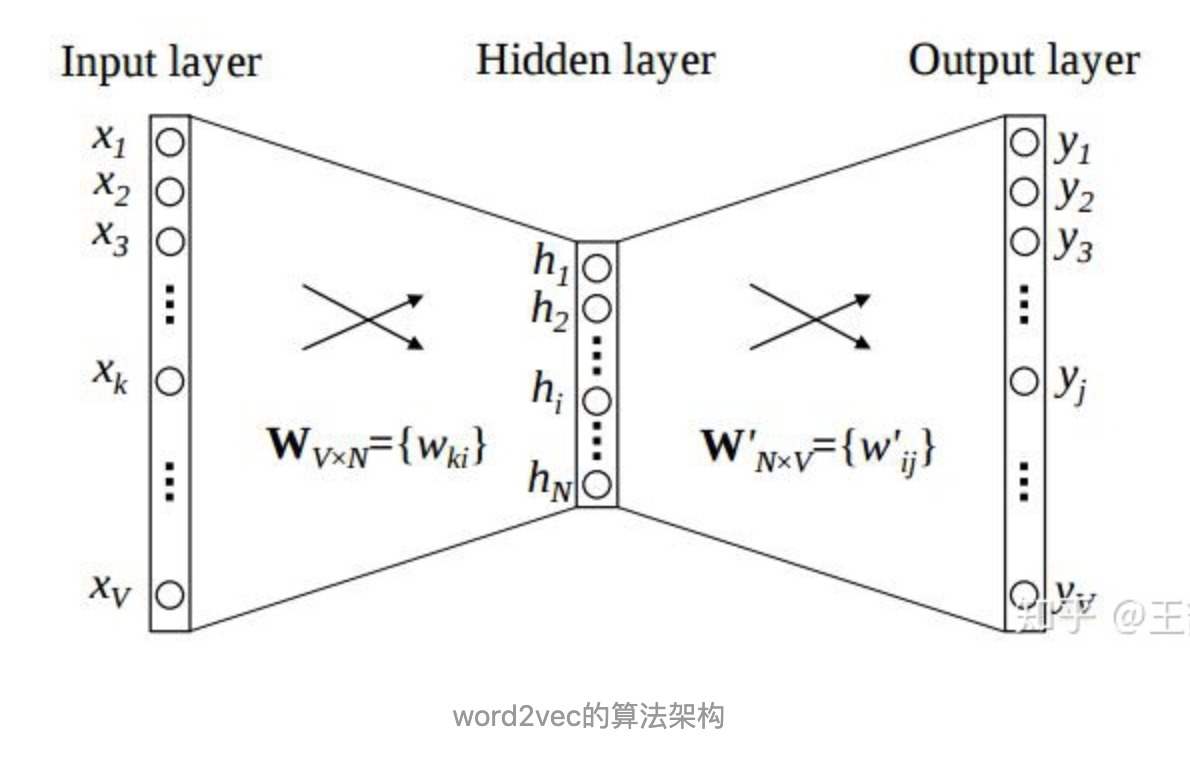
\includegraphics[width=.8\textwidth]{fig/Word2Vec_Algorithm_Structure.png}
\end{figure}

根据 $p(w_{t+j}|w_t)$ 的定义,我们可以把两个vector的乘积再套上一个softmax的形式转换成上面的神经网络架构(需要非常注意的一点是hidden layer的激活函数,大家要思考一下,到底是sigmoid函数还是普通的线性函数,为什么?)。在训练过程中我们就可以通过梯度下降的方式求解模型参数了。那么上文所说的输入向量表达就是input layer到hidden layer的权重矩阵$W_{V\times N}$ ,而输出向量表达就是hidden layer到output layer的权重矩阵$W'_{N\times V}$ 。

\textbf{那么到底什么是我们通常意义上所说的词向量 $v_w$ 呢?}

其实就是我们上面所说的输入向量矩阵 $W_{V\times N}$ 中每一行对应的权重向量。于是这个权重矩阵自然转换成了word2vec的lookup table。
\begin{figure}[H]
    \centering
    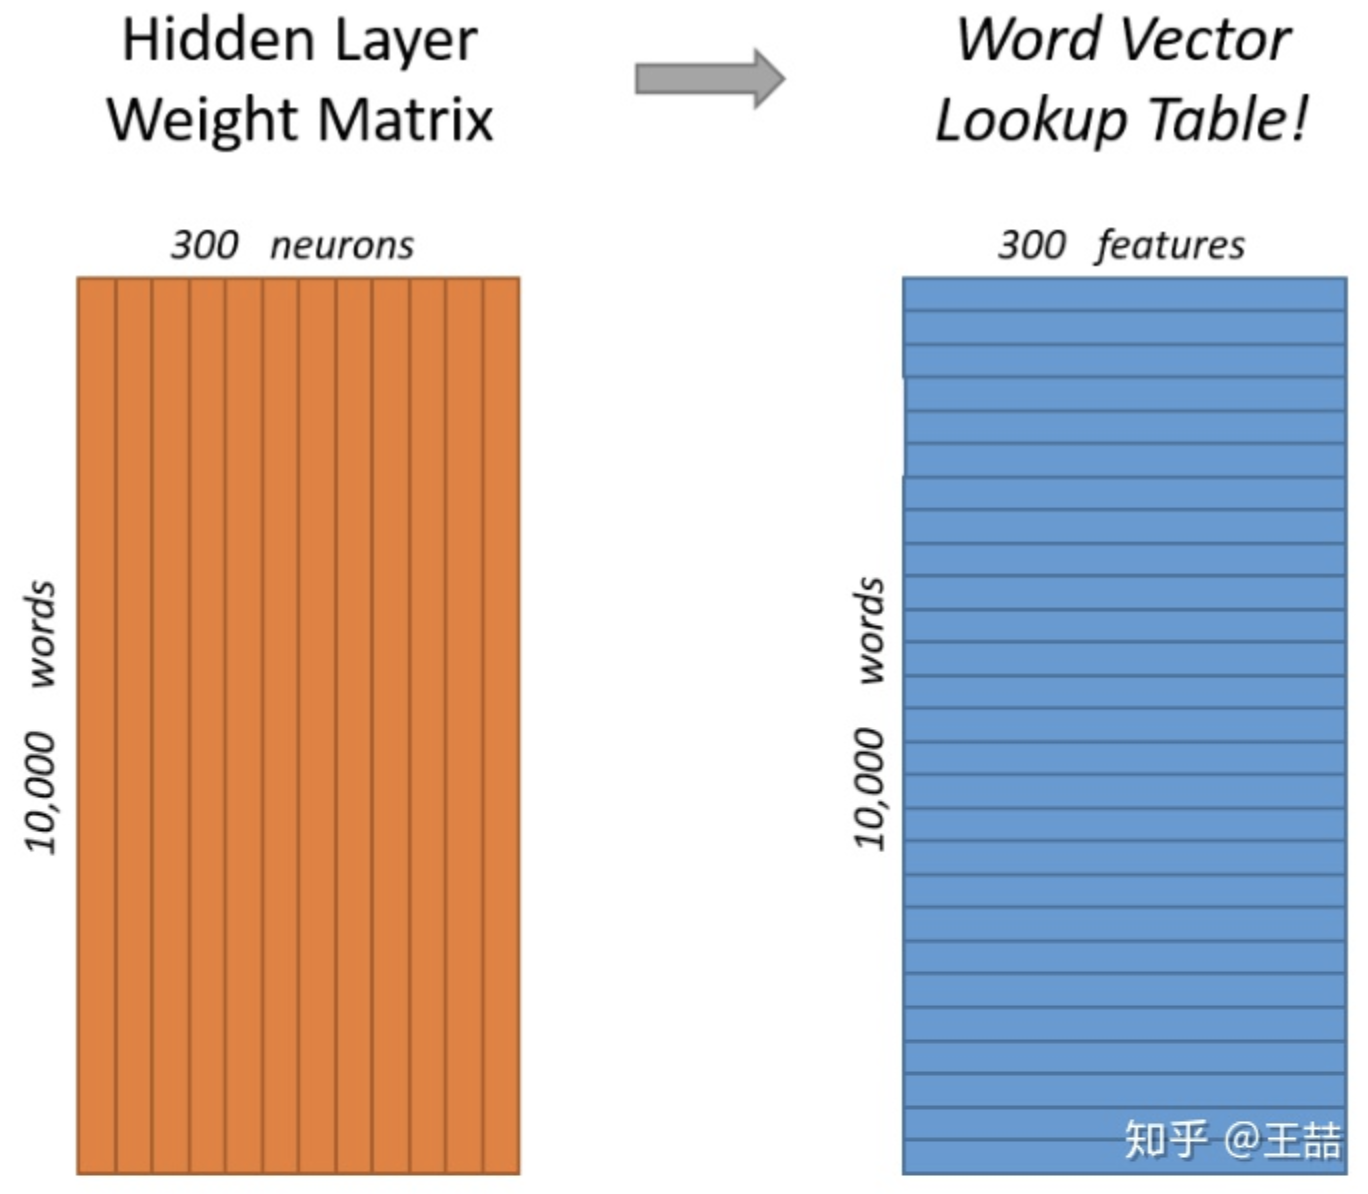
\includegraphics[width=.6\textwidth]{fig/Word2Vec_Lookup_Table.png}
\end{figure}

当然在训练word2vec的过程中还有很多工程技巧,比如用negative sampling或Hierarchical Softmax减少词汇空间过大带来的计算量,对高频词汇进行降采样避免对于这些低信息词汇的无谓计算等。在具体实现的时候最好参考Google的原文 Distributed Representations of Words and Phrases and their Compositionality

\subsection{从word2vec到item2vec}
在word2vec诞生之后,embedding的思想迅速从NLP领域扩散到几乎所有机器学习的领域,我们既然可以对一个序列中的词进行embedding,那自然可以对用户购买序列中的一个商品,用户观看序列中的一个电影进行embedding。而广告、推荐、搜索等领域用户数据的稀疏性几乎必然要求在构建DNN之前对user和item进行embedding后才能进行有效的训练。

具体来讲,如果item存在于一个序列中,item2vec的方法与word2vec没有任何区别。而如果我们摒弃序列中item的空间关系,在原来的目标函数基础上,自然是不存在时间窗口的概念了,取而代之的是item set中两两之间的条件概率:
$$
\frac{1}{K}\sum_{i=1}^K\sum_{j \neq i}^K \log{p(w_j|w_i)}
$$

具体可以参考item2vec的原文 Item2Vec:Neural Item Embedding for Collaborative Filtering

但embedding的应用又远不止于此,事实上,由于我们也可以把输出矩阵的列向量当作item embedding,这大大解放了我们可以用复杂网络生成embedding的能力。读过我专栏上一篇文章 YouTube深度学习推荐系统的十大工程问题 的同学肯定知道,YouTube在serve其candidate generation model的时候,只将最后softmax层的输出矩阵的列向量当作item embedding vector,而将softmax之前一层的值当作user embedding vector。在线上serving时不用部署整个模型,而是只存储user vector和item vector,再用最近邻索引进行快速搜索,这无疑是非常实用的embedding工程经验,也证明了我们可以用复杂网络生成user和item的embedding。

\begin{figure}[H]
    \centering
    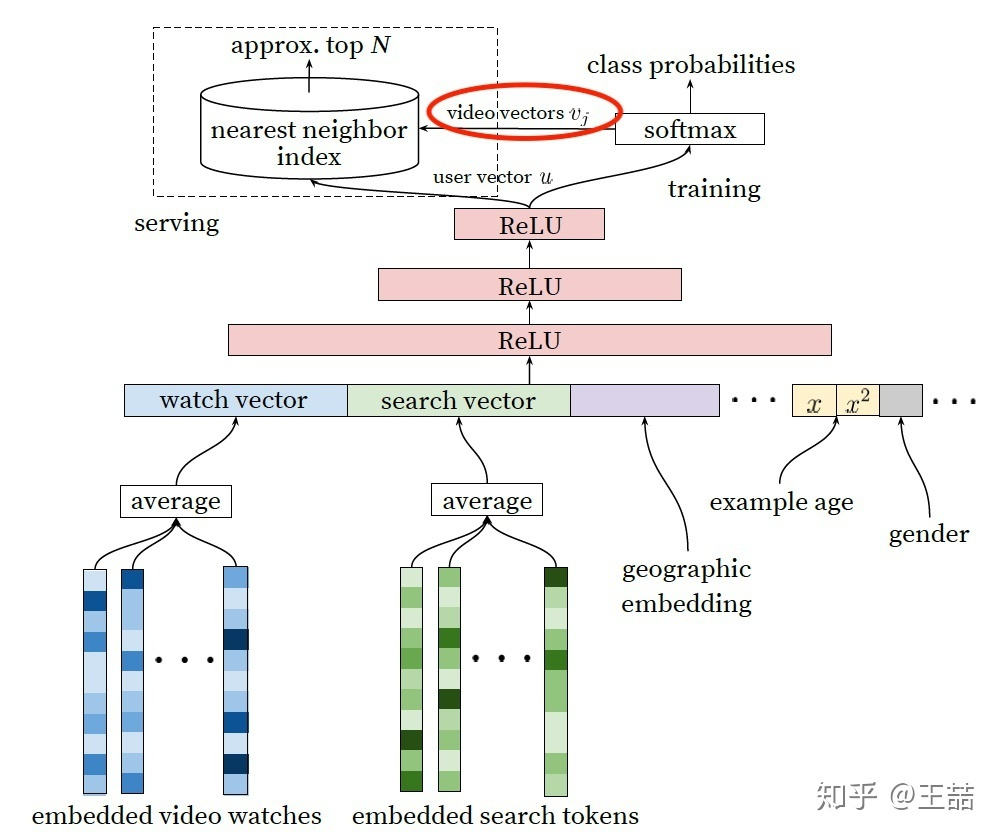
\includegraphics[width=.8\textwidth]{fig/Embedding_In_Youtube_2.jpg}
\end{figure}

KDD 2018 best paper Real-time Personalization using Embeddings for Search Ranking at Airbnb 也介绍了Airbnb的embedding最佳实践。

\section{Embedding在深度推荐系统中的3大应用方向
\cite{Three_Application_Of_Embedding_In_Reference_System}}

在深度学习推荐系统中,Embedding有三个主要的应用方向:
\begin{itemize}
\setlength{\itemsep}{0pt}
\setlength{\parsep}{0pt}
\setlength{\parskip}{0pt}
    \item 在深度学习网络中作为Embedding层,完成从高维稀疏特征向量到低维稠密特征向量的转换;
    \item 作为预训练的Embedding特征向量,与其他特征向量连接后一同输入深度学习网络进行训练;
    \item 通过计算用户和物品的Embedding相似度,Embedding可以直接作为推荐系统或计算广告系统的召回层或者召回方法之一;
\end{itemize}

\subsection{深度学习网络中的Embedding层}
由于高维稀疏特征向量天然不适合多层复杂神经网络的训练,因此如果使用深度学习模型处理高维稀疏特征向量,几乎都会在输入层到全连接层之间加入Embedding层完成高维稀疏特征向量到低维稠密特征向量的转换。典型的例子是微软的Deep Crossing模型和Google的Wide\&Deep模型的深度部分。
\begin{figure}[H]
    \centering
    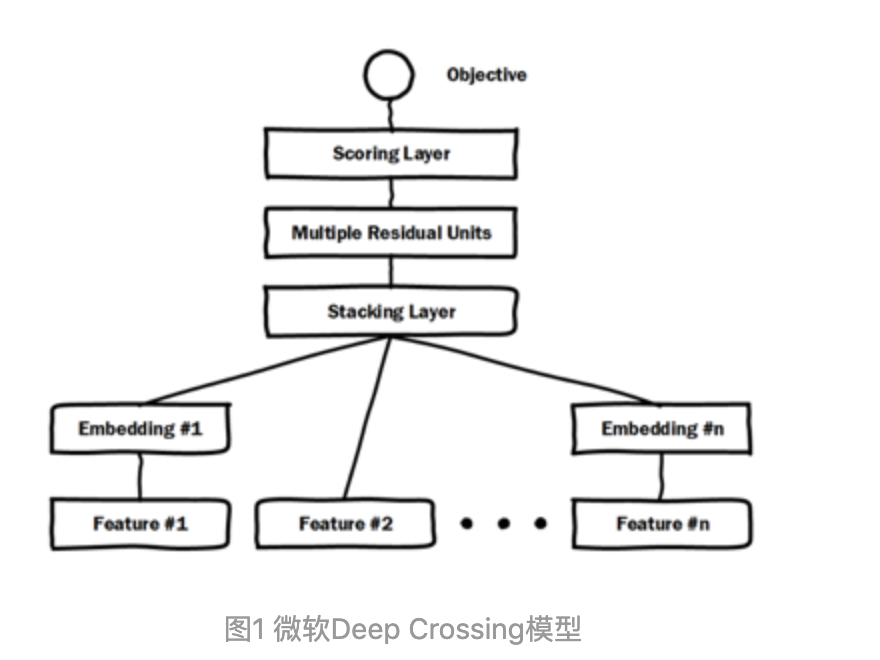
\includegraphics[width=.8\textwidth]{fig/Microsoft_Deep_Crossing_Strucure.png}
\end{figure}
\begin{figure}[H]
    \centering
    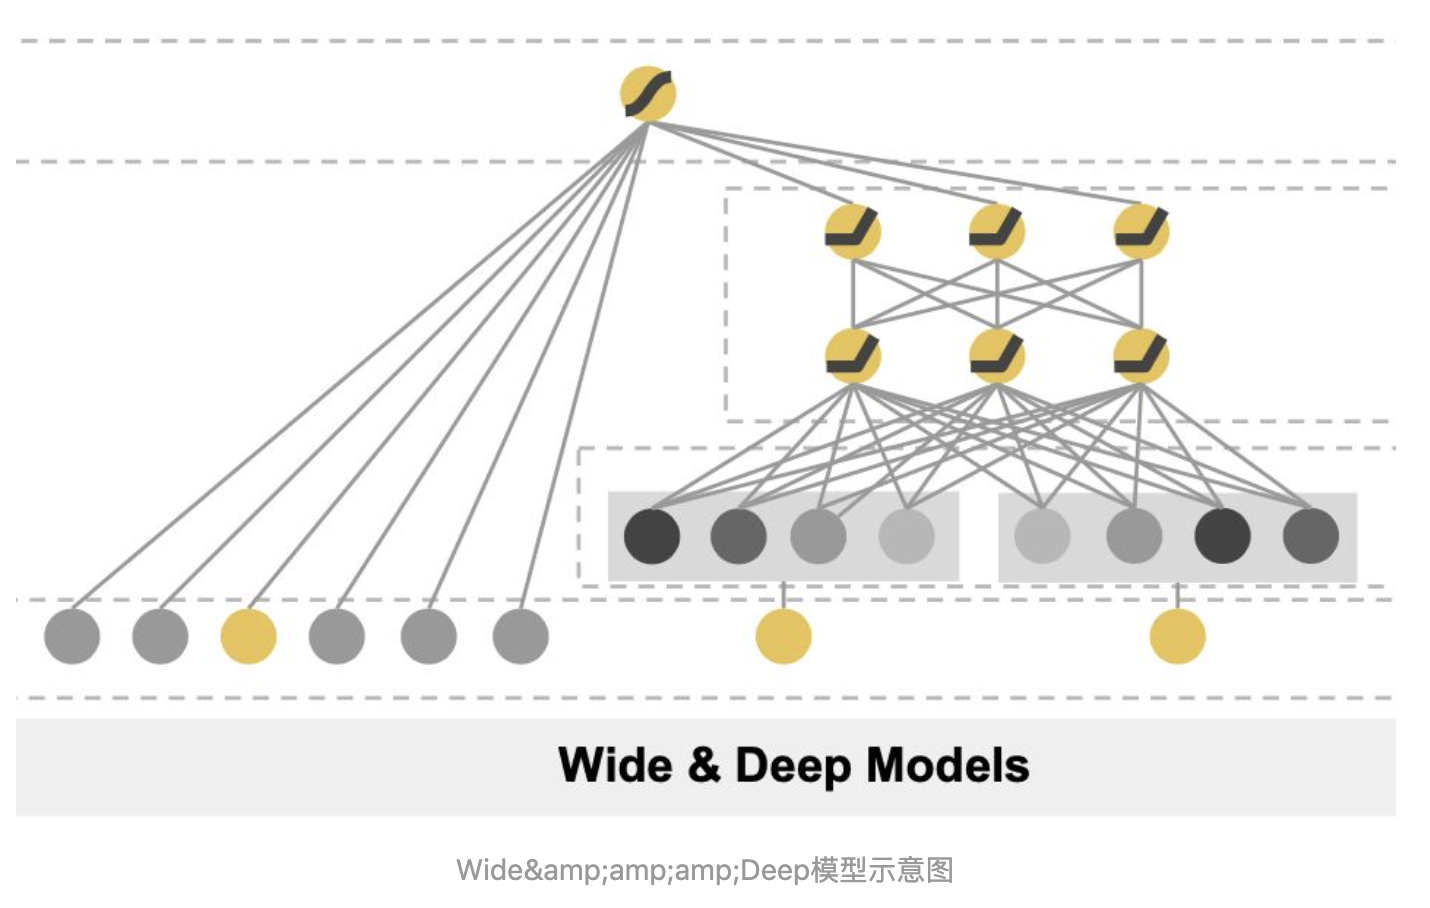
\includegraphics[width=.8\textwidth]{fig/Wide_Deep_Structure.png}
\end{figure}

图1中可以清晰的看到Deep Crossing模型中的Embedding层将每一个Feature转换成稠密向量,图2Wide\&Deep模型中Deep部分的Dense Embeddings层同样将稀疏特征向量进行转换。广义来说,Embedding层的结构可以比较复杂,只要完成高维向量的降维就可以了,但一般为了节省训练时间,深度神经网络中的Embedding层是一个高维向量向低维向量的直接映射(如图3)。
\begin{figure}[H]
    \centering
    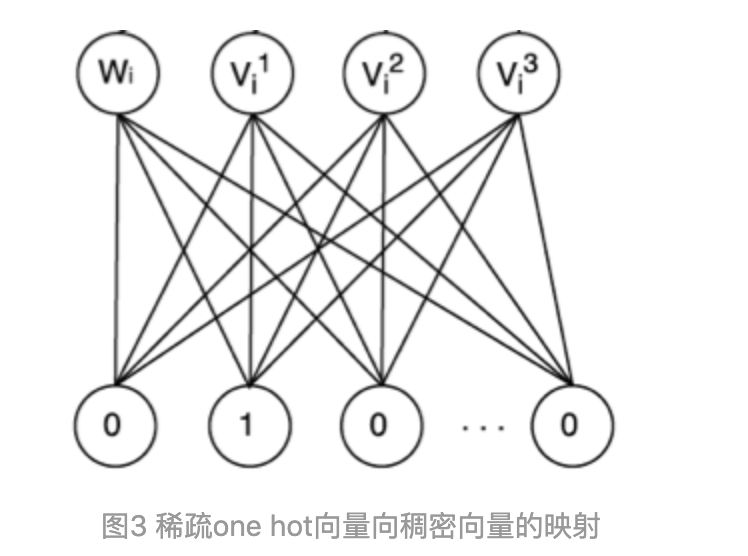
\includegraphics[width=.5\textwidth]{fig/Embedding_From_One_Hot_Example.png}
\end{figure}

一般来说,推荐系统的输入向量中包含大量稀疏的 one hot 特征,图3展示了典型的稀疏向量向稠密embedding向量的最简单的embedding层结构。

用矩阵的形式表达Embedding层,本质上是求解一个 m(输入高维稀疏向量的维度) x n(输出稠密向量的维度)维的权重矩阵的过程。如果输入向量是 one-hot 特征向量的话,权重矩阵中的列向量即为相应维度one-hot特征的embedding向量。

将Embedding层与整个深度学习网络整合后一同进行训练是理论上最优的选择,因为上层梯度可以直接反向传播到输入层,模型整体是自洽和统一的。但这样做的缺点同样显而易见的,由于Embedding层输入向量的维度甚大,Embedding层的加入会拖慢整个神经网络的收敛速度。

\begin{framed}
这里可以做一个简单的计算。假设输入层维度是100,000,embedding输出维度是32,上层再加5层32维的全连接层,最后输出层维度是10,那么输出层到embedding层的参数数量是32*100,000= 3,200,000,其余所有层的参数总数是 (32*32)*4+32*10=4416。那么embedding层的权重总数占比是 3,200,000 / (3,200,000 + 4416) = 99.86\%。
\end{framed}

也就是说embedding层的权重占据了整个网络权重的绝大部分。那么训练过程可想而知,大部分的训练时间和计算开销都被Embedding层所占据。正因为这个原因,Embedding层往往采用预训练的方式完成。

\subsection{Embedding的预训练方法}
通过上面对Embedding层的介绍,同学们肯定已经知道Embedding层的训练开销是巨大的。为了解决这个问题,Embedding的训练往往独立于深度学习网络进行。在得到稀疏特征的稠密表达之后,再与其他特征一起输入神经网络进行训练。典型的采用Embedding预训练方法的模型是FNN(如图4)。
\begin{figure}[H]
    \centering
    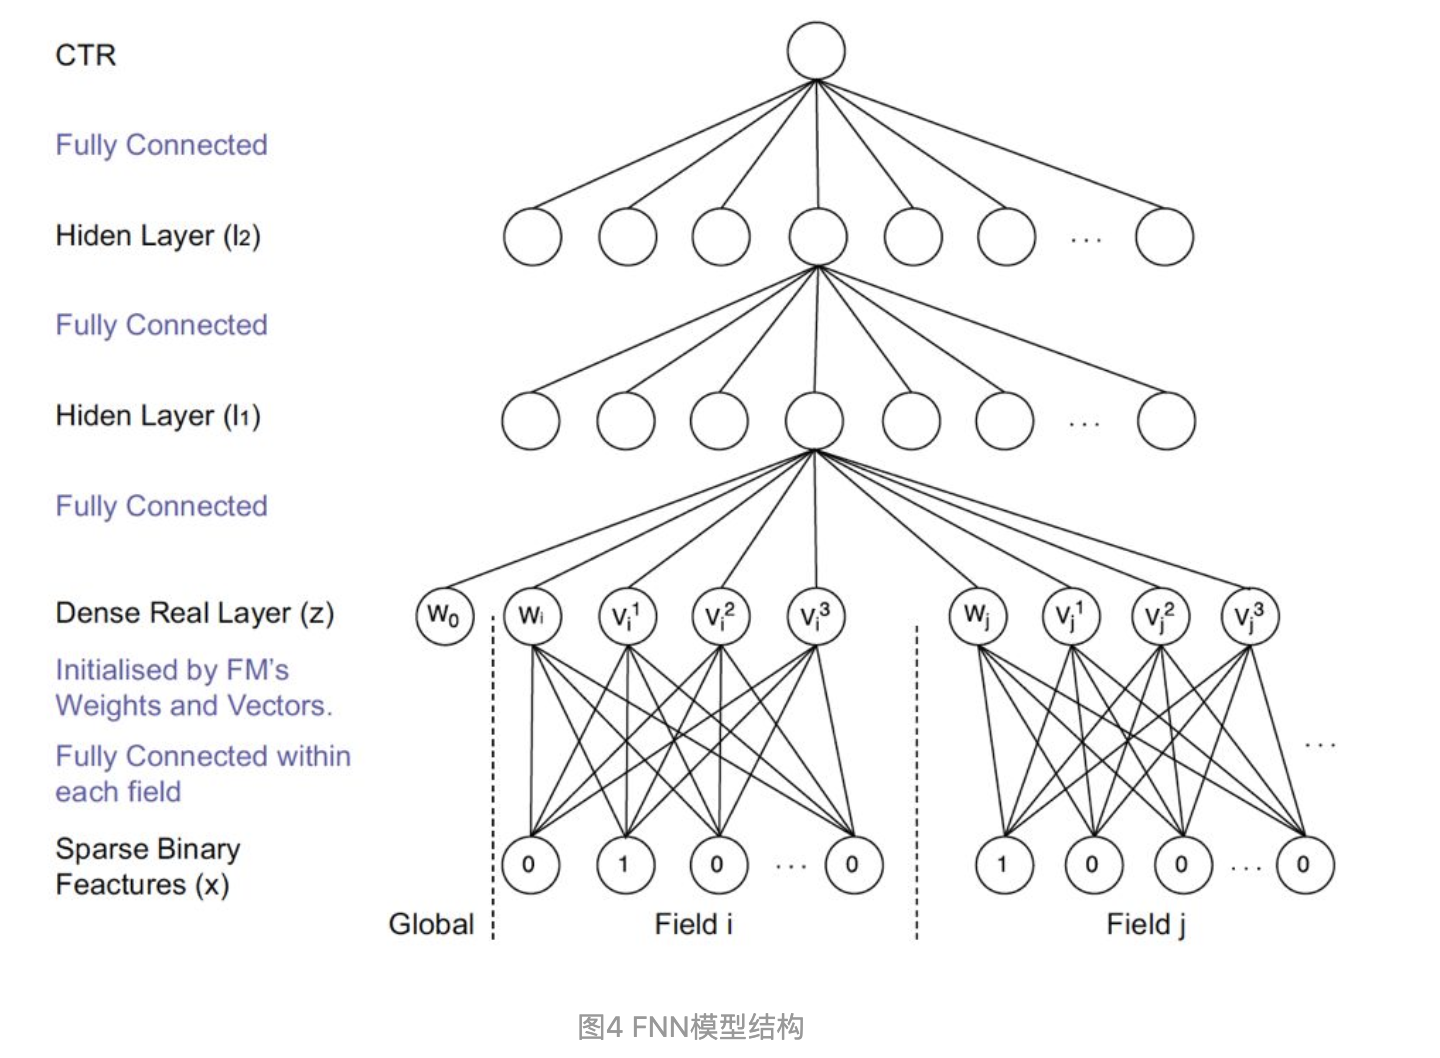
\includegraphics[width=.8\textwidth]{fig/FNN_Structure.png}
\end{figure}

FNN利用了FM训练得到的物品向量,作为Embedding层的初始化权重,从而加快了整个网络的收敛速度。在实际工程中,直接采用FM的物品向量作为Embedding特征向量输入到后续深度学习网络也是可行的办法。

再延伸一点讲,Embedding的本质是建立高维向量到低维向量的映射,而“映射”的方法并不局限于神经网络,实质上可以是任何异构模型,这也是Embedding预训练的另一大优势,就是可以采用任何传统降维方法,机器学习模型,深度学习网络完成embedding的生成。

典型的例子是2013年Facebook提出的著名的GBDT+LR的模型,其中GBDT的部分本质上也是完成了一次特征转换,可以看作是利用GBDT模型完成Embedding预训练之后,将Embedding输入单层神经网络进行CTR预估的过程。

\begin{figure}[H]
    \centering
    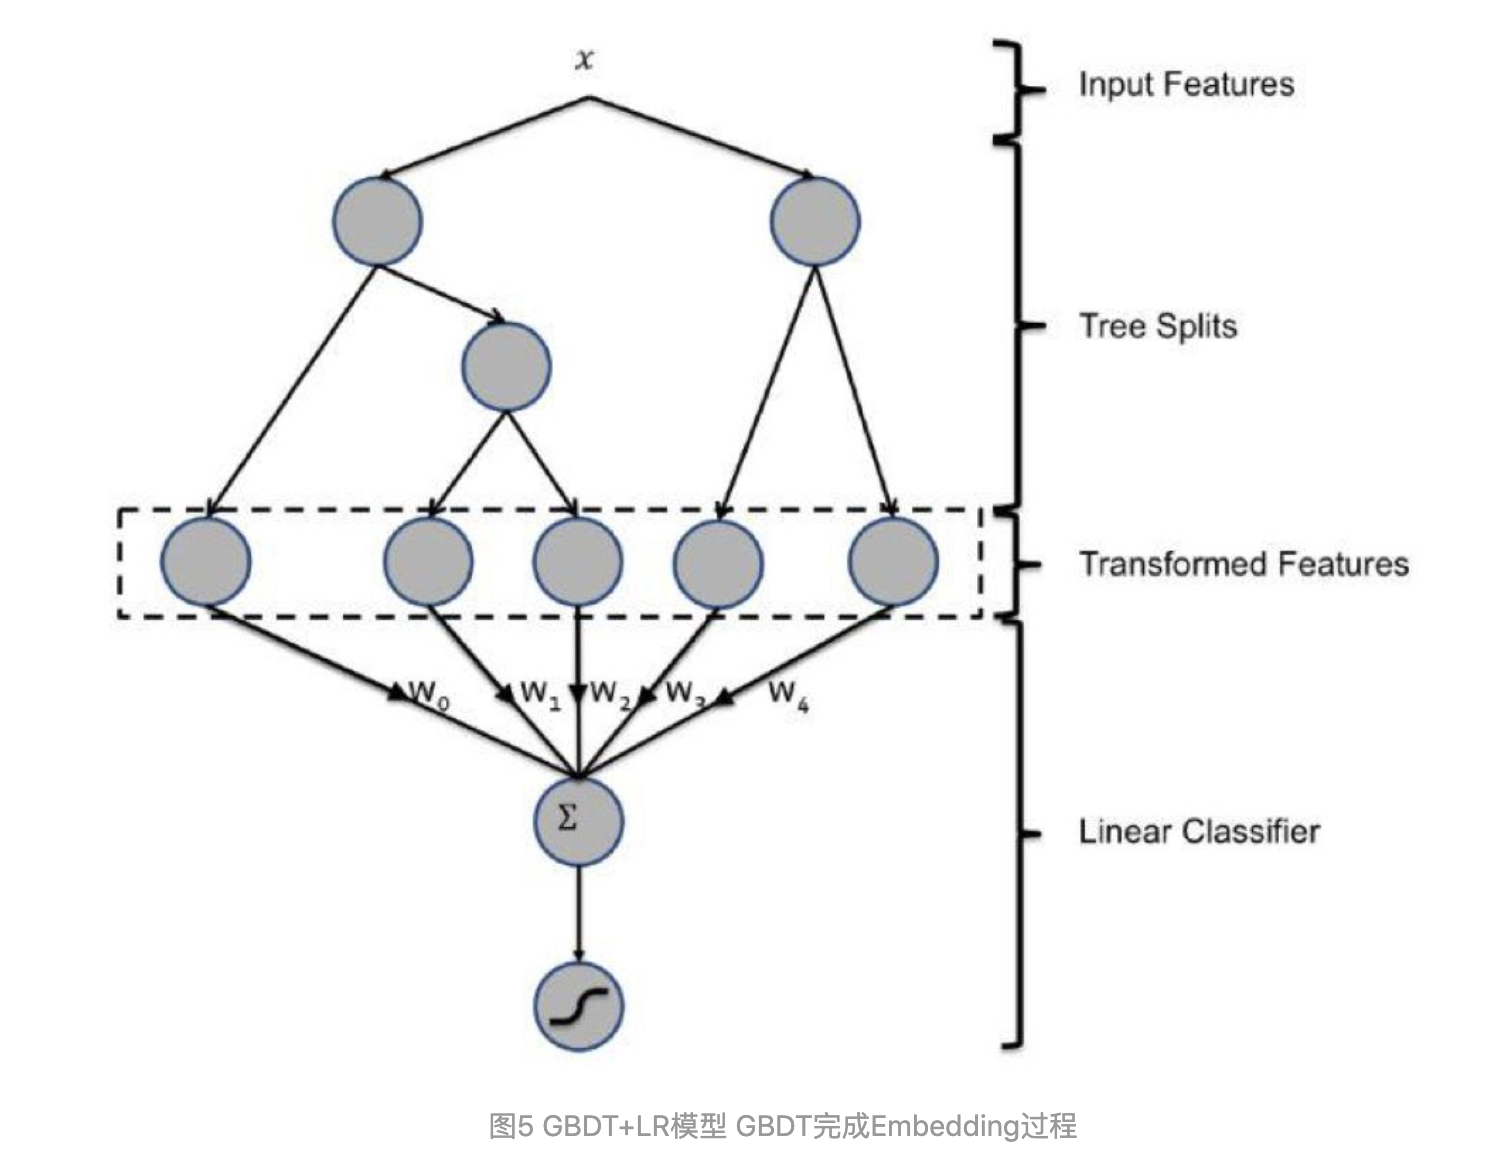
\includegraphics[width=1\textwidth]{fig/Embedding_GBDT_LR.png}
\end{figure}

2015年以来,随着大量Graph Embedding技术的发展,Embedding本身的表达能力进一步增强,而且能够将各类特征全部融合进Embedding之中,这使Embedding本身成为非常有价值的特征。这些特点都使Embedding预训练成为更被青睐的技术途径。

诚然,将Embedding过程与深度网络的训练过程割裂,必然会损失一定的信息,但训练过程的独立也带来了训练灵活性的提升。举例来说,由于物品或用户的Embedding天然是比较稳定的(因为用户的兴趣、物品的属性不可能在几天内发生巨大的变化),Embedding的训练频率其实不需要很高,甚至可以降低到周的级别,但上层神经网络为了尽快抓住最新的正样本信息,往往需要高频训练甚至实时训练。使用不同的训练频率更新Embedding模型和神经网络模型,是训练开销和模型效果二者之间权衡后的最优方案。

\subsection{embedding作为推荐系统或计算广告系统的召回层}
随着Embedding技术的进步,Embedding自身的表达能力也逐步增强,利用Embedding向量的相似性,直接将Embedding作为推荐系统召回层的方案越来越多的被采用。其中Youtube推荐系统召回层的解决方案是典型的做法。
\begin{figure}[H]
    \centering
    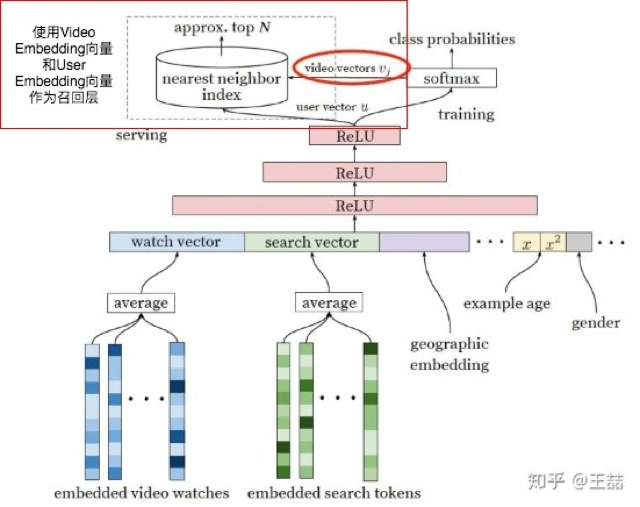
\includegraphics[width=1\textwidth]{fig/Embedding_In_Youtube.jpg}
\end{figure}

我曾经在文章《重读Youtube深度学习推荐系统论文,字字珠玑,惊为神文》中介绍过了Youtube利用深度学习网络生成Video Embedding和User Embedding的方法。利用最终的Softmax层的权重矩阵,每个Video对应的列向量就是其Item Embedding,而Softmax前一层的输出就是User Embedding。在模型部署过程中,没有必要部署整个深度学习网络来完成从原始特征向量到最终输出的预测过程,只需要将User Embedding和Item Embedding存储到线上内存数据库,通过内积运算再排序的方法就可以得到item的排名。这大大加快了召回层的召回效率。

\subsection{总结}
事实上,除了上述的三种主要的Embedding应用方向,业界对于Embedding的创新性研究不仅没有停止,而且有愈演愈烈之势,阿里的EGES,Pinterest的GNN应用,Airbnb基于Embedding的搜索模型等大量表达能力非常强的Embedding方法的诞生,使Embedding本身就已经成为了优秀的CTR模型和推荐系统模型。作为计算广告和推荐系统领域的从业者,无论如何强调Embedding的重要性都不过分。

\section{深度学习中的Graph Embedding方法
\cite{Graph_Embedding_In_Deep_Learning}}
\begin{itemize}
\setlength{\itemsep}{0pt}
\setlength{\parsep}{0pt}
\setlength{\parskip}{0pt}
    \item Graph Embedding是推荐系统、计算广告领域最近非常流行的做法,是从word2vec等一路发展而来的Embedding技术的最新延伸;
    \item 已经有很多大厂将Graph Embedding应用于实践后取得了非常不错的线上效果;
\end{itemize}

word2vec和由其衍生出的item2vec是embedding技术的基础性方法,但二者都是建立在“序列”样本(比如句子、推荐列表)的基础上的。而在互联网场景下,数据对象之间更多呈现的是图结构。典型的场景是由用户行为数据生成的和物品全局关系图(图1),以及加入更多属性的物品组成的知识图谱(图2)。
\begin{figure}[H]
    \centering
    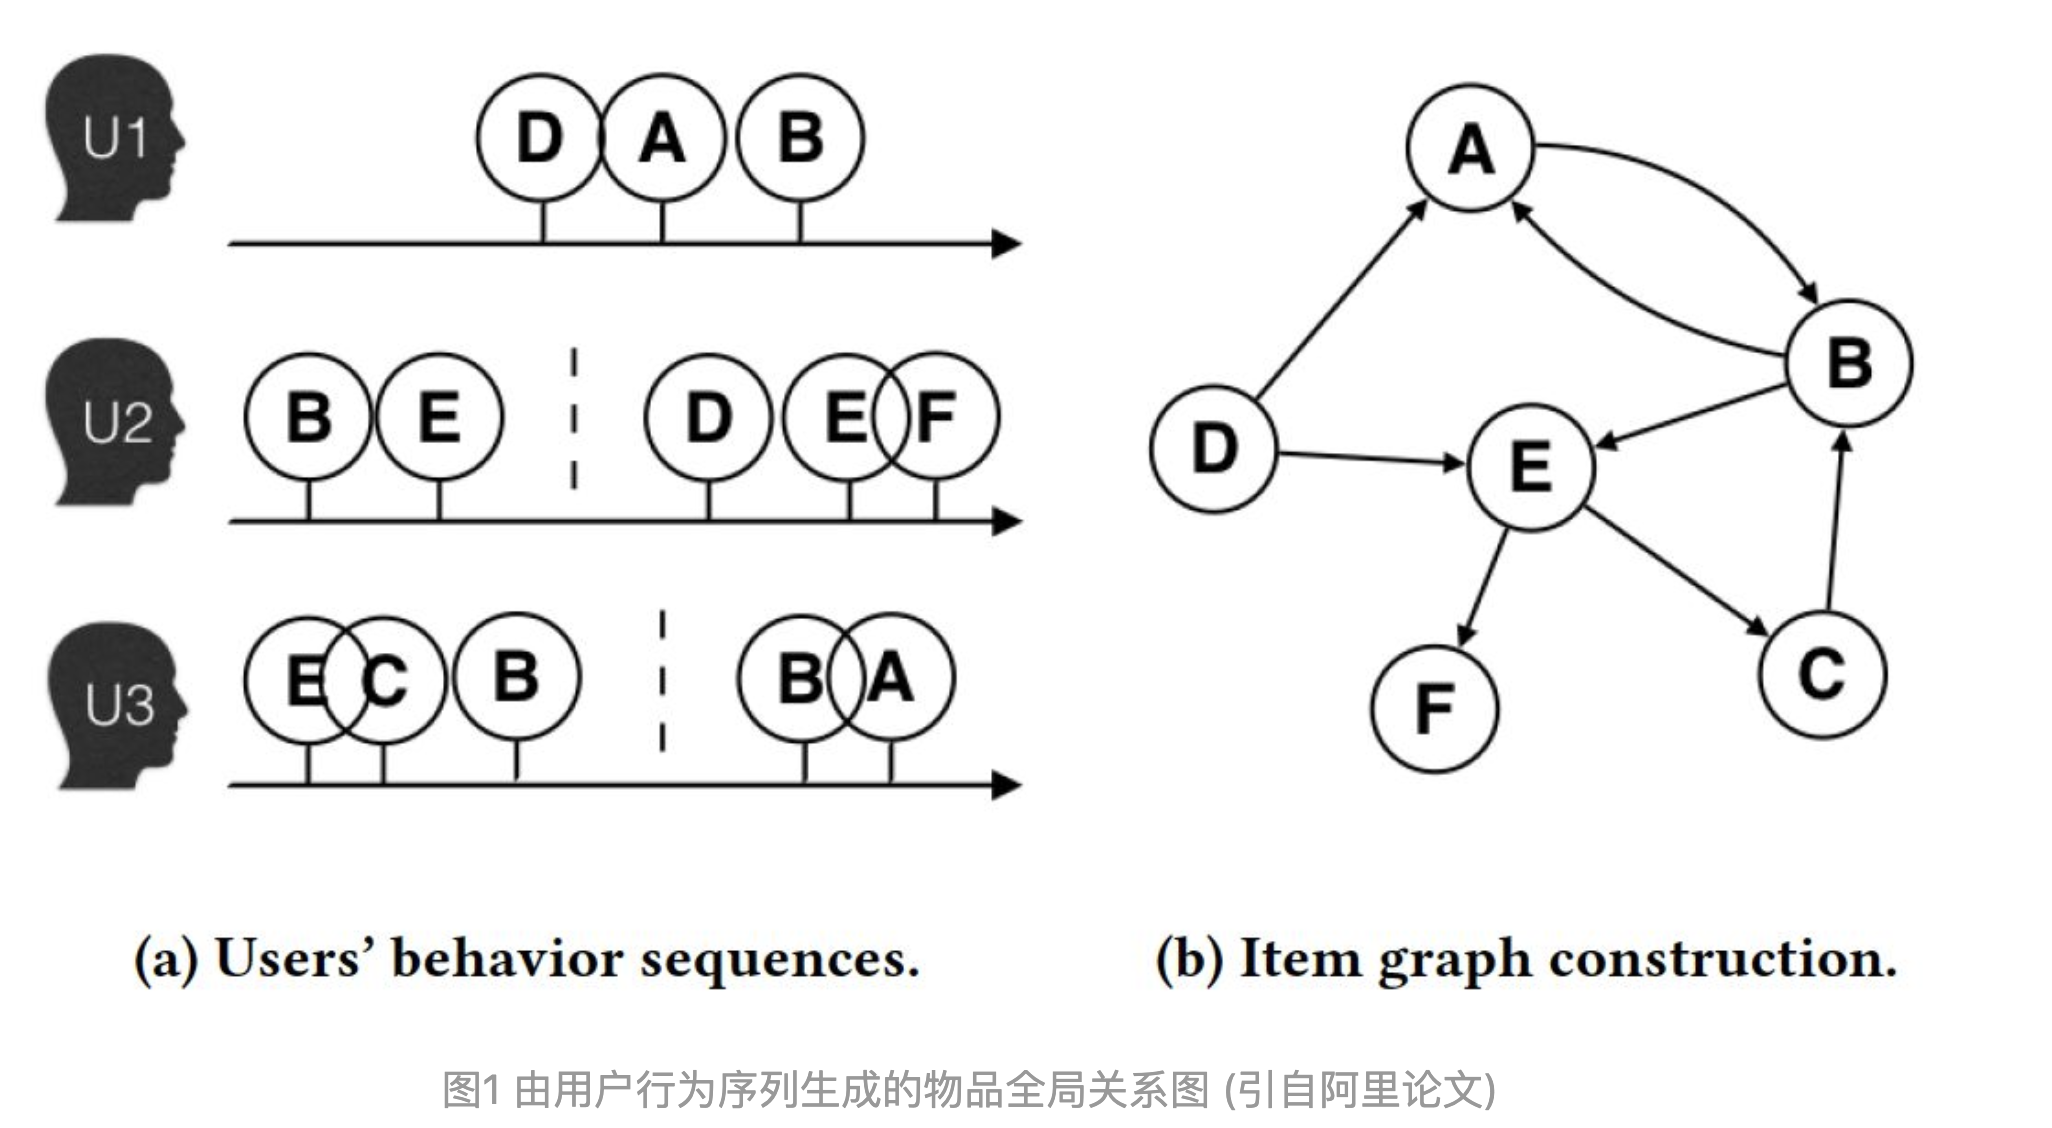
\includegraphics[width=.6\textwidth]{fig/Graph_Embedding_User_Activity_Graph.png}
\end{figure}

\begin{figure}[H]
    \centering
    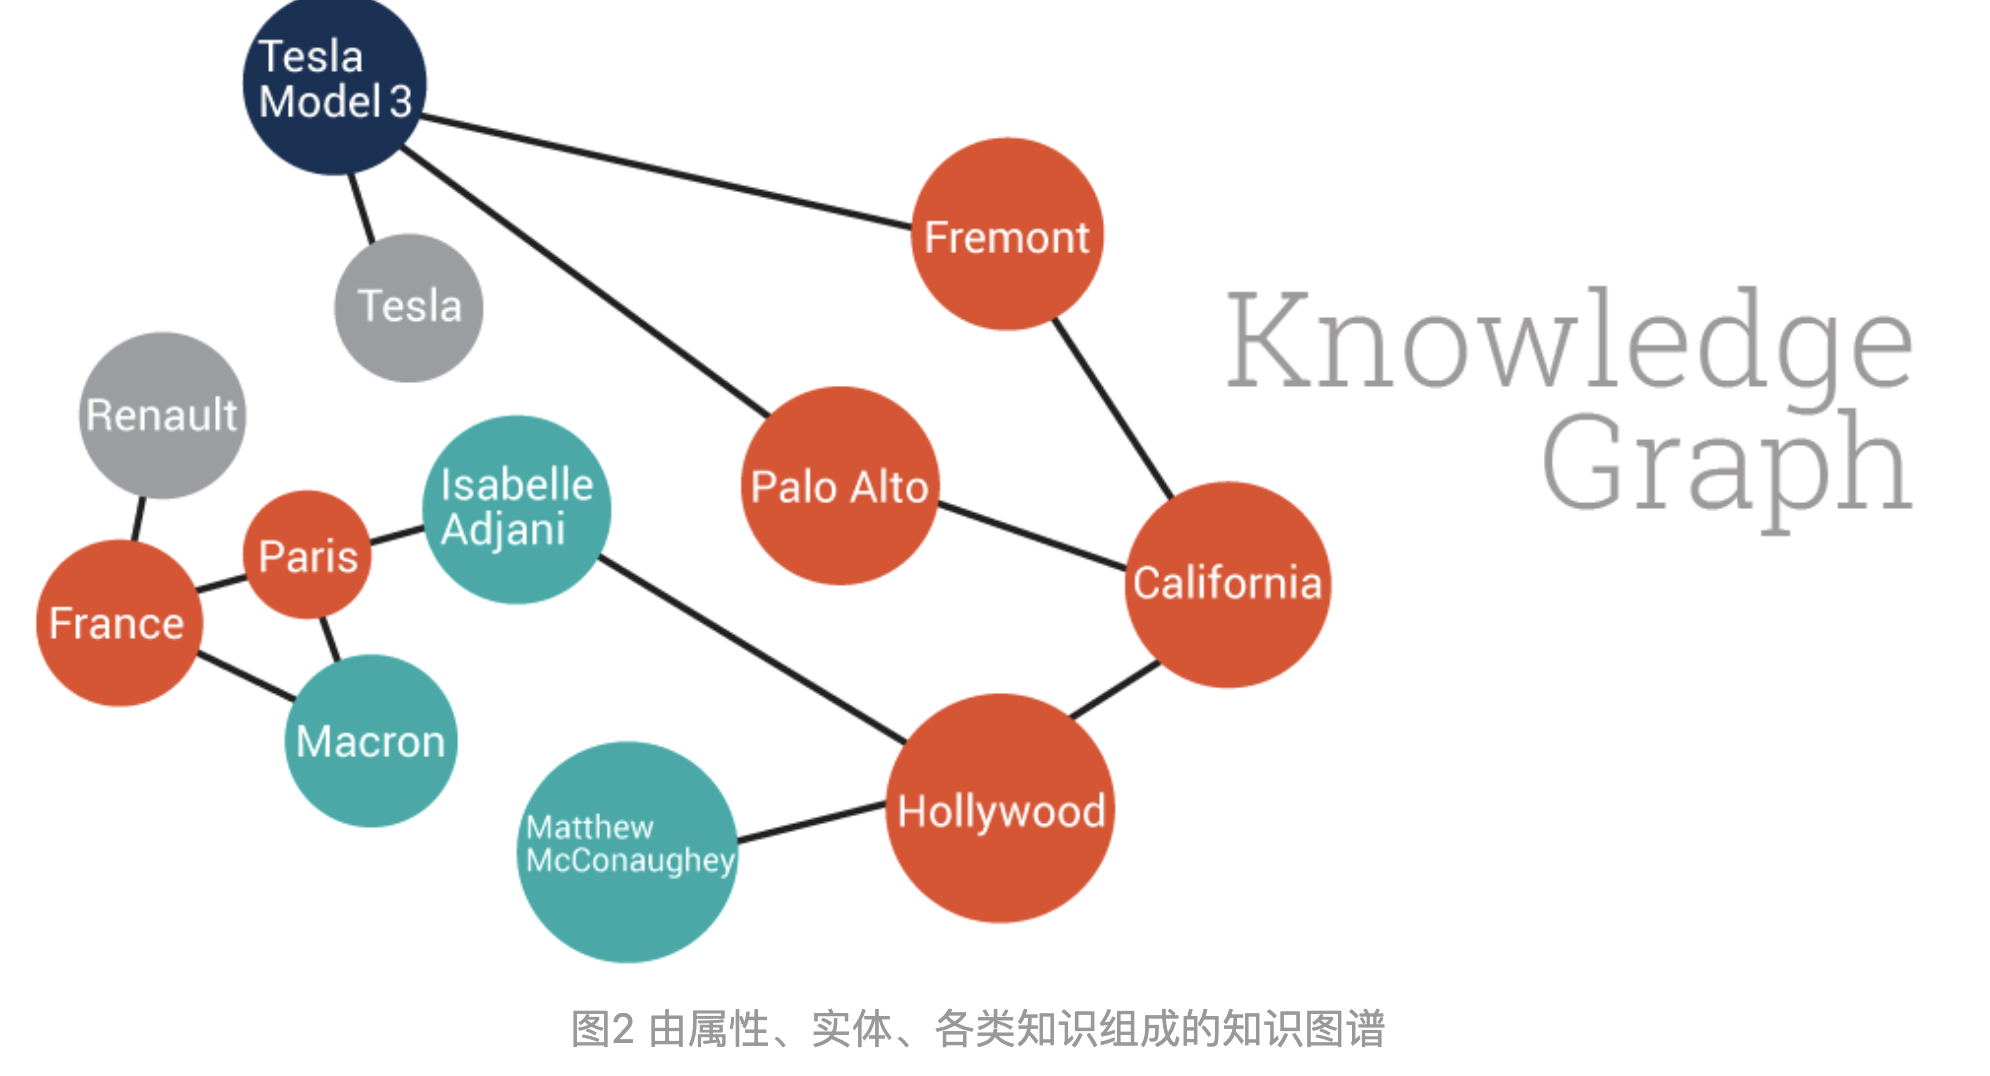
\includegraphics[width=.6\textwidth]{fig/Graph_Embedding_Knowledge_Graph.png}
\end{figure}

在面对图结构的时候,传统的序列embedding方法就显得力不从心了。在这样的背景下,对图结构中间的节点进行表达的graph embedding成为了新的研究方向,并逐渐在深度学习推荐系统领域流行起来。

\subsection{经典的Graph Embedding方法——DeepWalk}
早期影响力较大的graph embedding方法是2014年提出的DeepWalk,它的主要思想是在由物品组成的图结构上进行\textbf{随机游走,产生大量物品序列},然后将这些物品序列作为训练样本输入word2vec进行训练,得到物品的embedding。图3用图示的方法展现了DeepWalk的过程。
\begin{figure}[H]
    \centering
    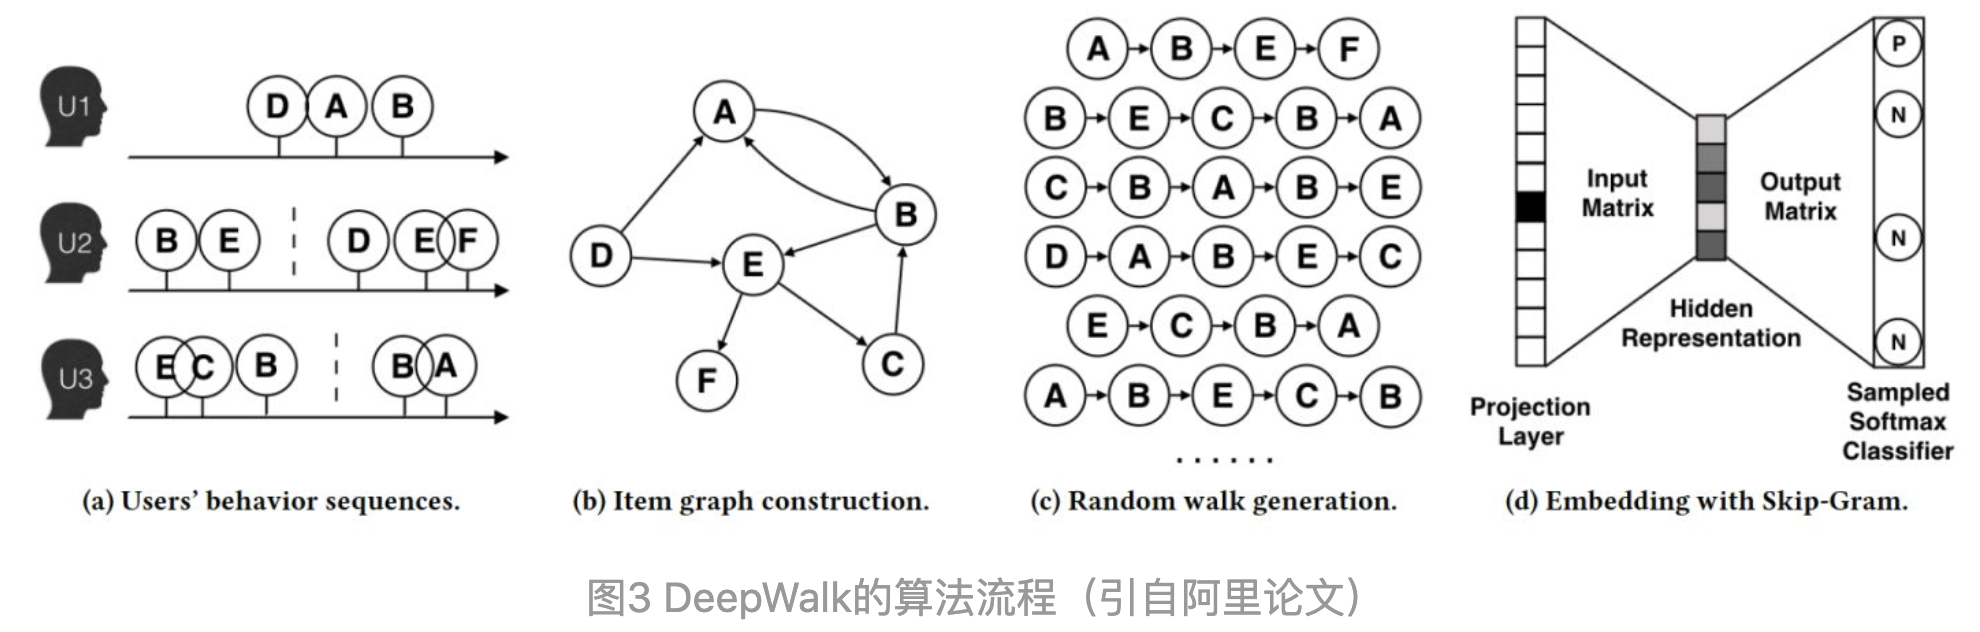
\includegraphics[width=.6\textwidth]{fig/Graph_Embedding_Deep_Walk_Example.png}
\end{figure}

如图3,整个DeepWalk的算法流程可以分为四步:
\begin{itemize}
\setlength{\itemsep}{0pt}
\setlength{\parsep}{0pt}
\setlength{\parskip}{0pt}
    \item 图a展示了原始的用户行为序列;
    \item 图b基于这些用户行为序列构建了物品相关图,可以看出,物品A,B之间的边产生的原因就是因为用户U1先后购买了物品A和物品B,所以产生了一条由A到B的有向边。如果后续产生了多条相同的有向边,则有向边的权重被加强。在将所有用户行为序列都转换成物品相关图中的边之后,全局的物品相关图就建立起来了;
    \item 图c采用随机游走的方式随机选择起始点,重新产生物品序列;
    \item 图d最终将这些物品序列输入word2vec模型,生成最终的物品Embedding向量。
\end{itemize}

在上述DeepWalk的算法流程中,核心是第三步,其中唯一需要形式化定义的是随机游走的跳转概率,也就是到达节点vi后,下一步遍历vi的临接点vj的概率。如果物品的相关图是有向有权图,那么从节点vi跳转到节点vj的概率定义如下:
\begin{figure}[H]
    \centering
    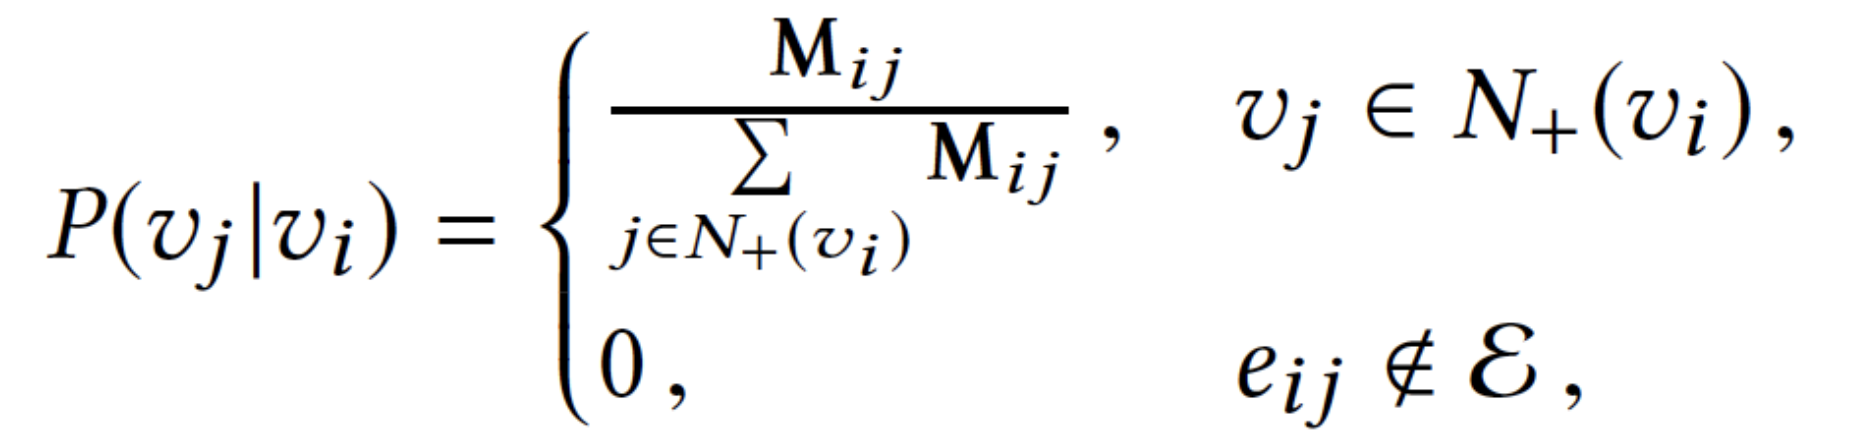
\includegraphics[width=.6\textwidth]{fig/Graph_Embedding_Deep_Walk_Trans_Prob.png}
\end{figure}

其中N+(vi)是节点vi所有的出边集合,Mij是节点vi到节点vj边的权重。

如果物品相关图是无相无权重图,那么跳转概率将是上面公式的一个特例,即权重Mij将为常数1,且N+(vi)应是节点vi所有“边”的集合,而不是所有“出边”的集合。

\subsection{DeepWalk的进一步改进——Node2vec}
2016年,斯坦福大学在DeepWalk的基础上更进一步,通过调整随机游走权重的方法使graph embedding的结果在网络的同质性(homophily)和结构性(structural equivalence)中进行权衡权衡。

具体来讲,网络的“同质性”指的是距离相近节点的embedding应该尽量近似,如图4,节点u与其相连的节点s1、s2、s3、s4的embedding表达应该是接近的,这就是“同质性“的体现。
\begin{figure}[H]
    \centering
    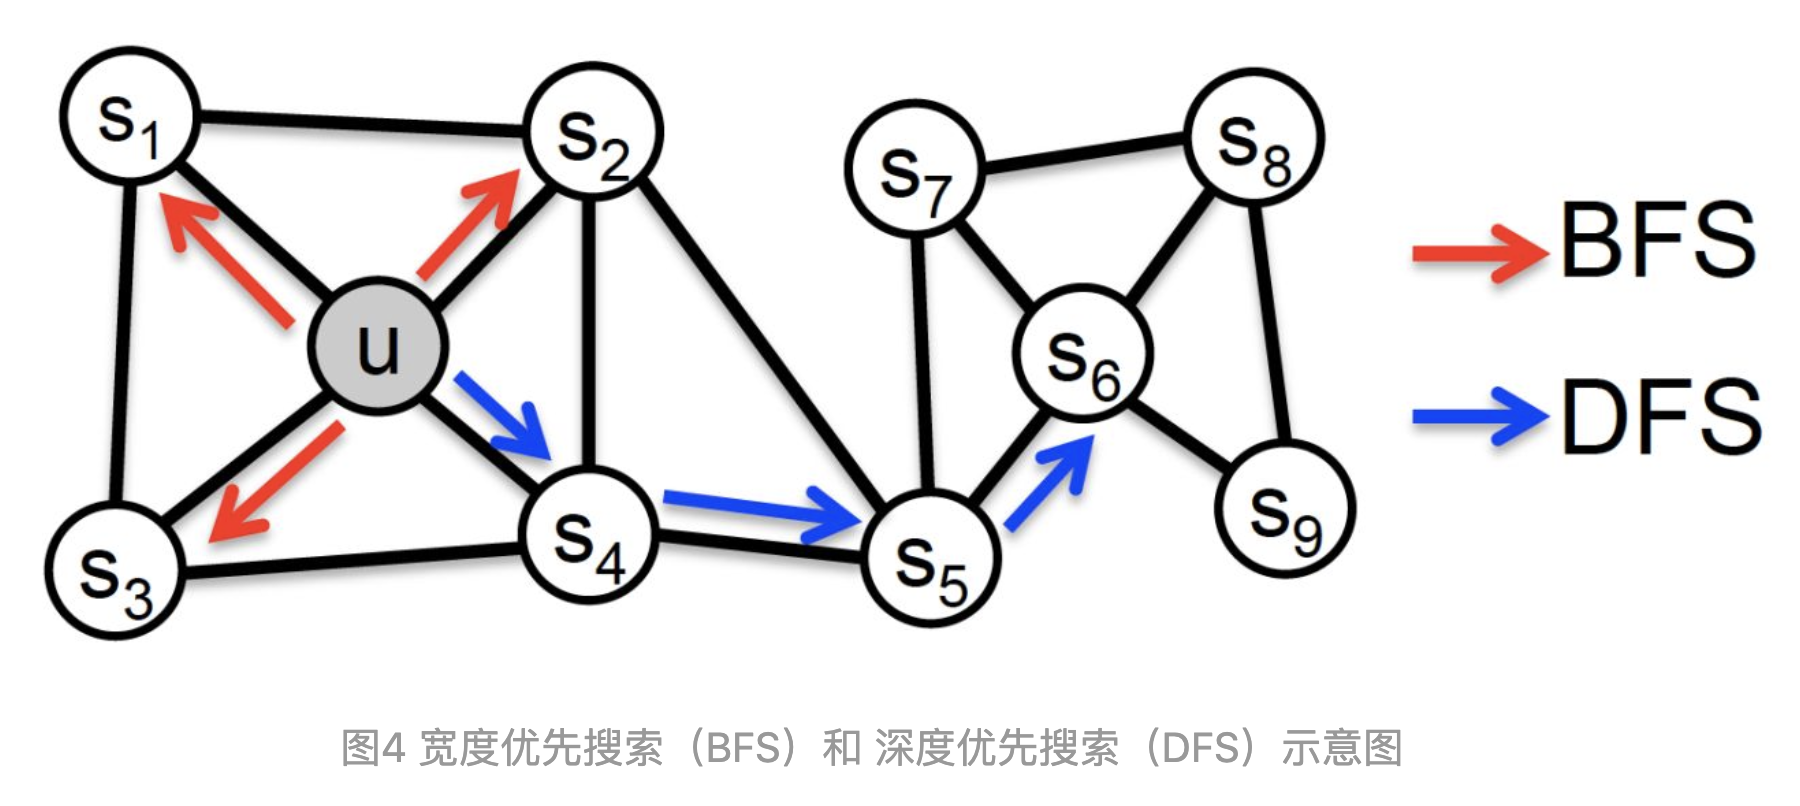
\includegraphics[width=.6\textwidth]{fig/Graph_Embedding_BFS_DFS.png}
\end{figure}

为了使Graph Embedding的结果能够表达网络的同质性,在随机游走的过程中,需要让游走的过程更倾向于宽度优先搜索(BFS),因为BFS更喜欢游走到跟当前节点有直接连接的节点上,因此就会有更多同质性信息包含到生成的样本序列中,从而被embedding表达;另一方面,为了抓住网络的结构性,就需要随机游走更倾向于深度优先搜索(DFS),因为DFS会更倾向于通过多次跳转,游走到远方的节点上,使得生成的样本序列包含更多网络的整体结构信息。(通过 
@张备
 同学的提醒,这里其实是写反了,BFS应该反映了结构性,DFS反而反应了同质性,大家可以深度思考一下这是为什么,欢迎在评论区讨论)

那么在node2vec算法中,是怎样控制BFS和DFS的倾向性的呢?主要是通过节点间的跳转概率。图5显示了node2vec算法从节点t跳转到节点v后,下一步从节点v跳转到周围各点的跳转概率。
\begin{figure}[H]
    \centering
    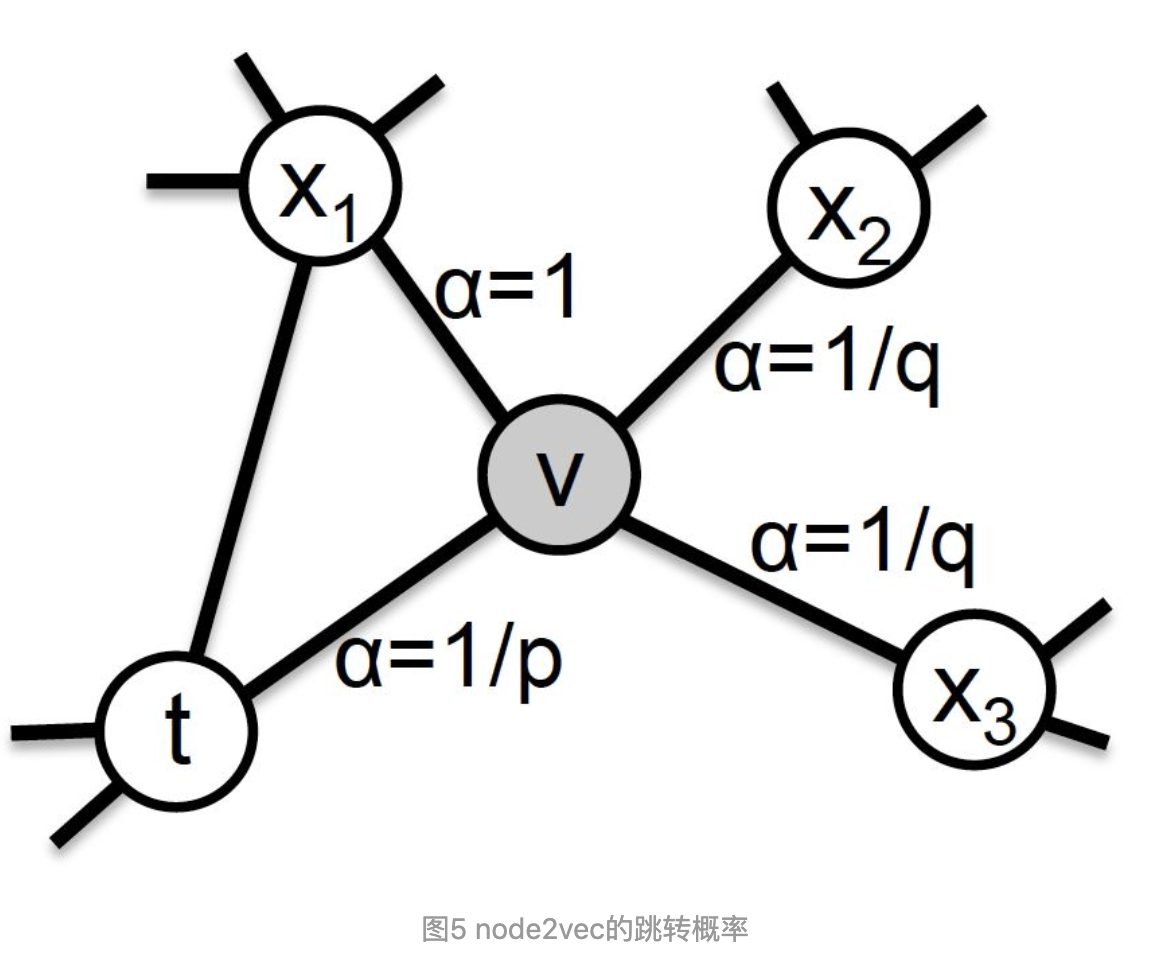
\includegraphics[width=.6\textwidth]{fig/Graph_Embedding_Node2Vec_Trans_Prob.png}
\end{figure}

形式化来讲,从节点v跳转到下一个节点x的概率为
\begin{figure}[H]
    \centering
    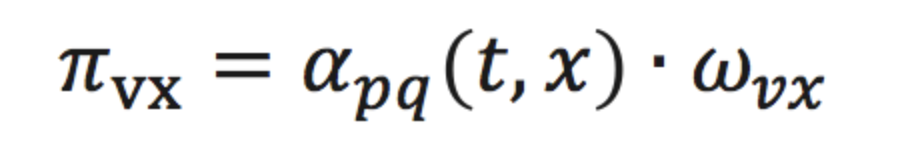
\includegraphics[width=.6\textwidth]{fig/Graph_Embedding_Node2Vec_Trans_Prob_2.png}
\end{figure}

其中$w_{vx}$ 是边vx的权重, $\alpha_{pq}(t,x)$ 的定义如下:
\begin{figure}[H]
    \centering
    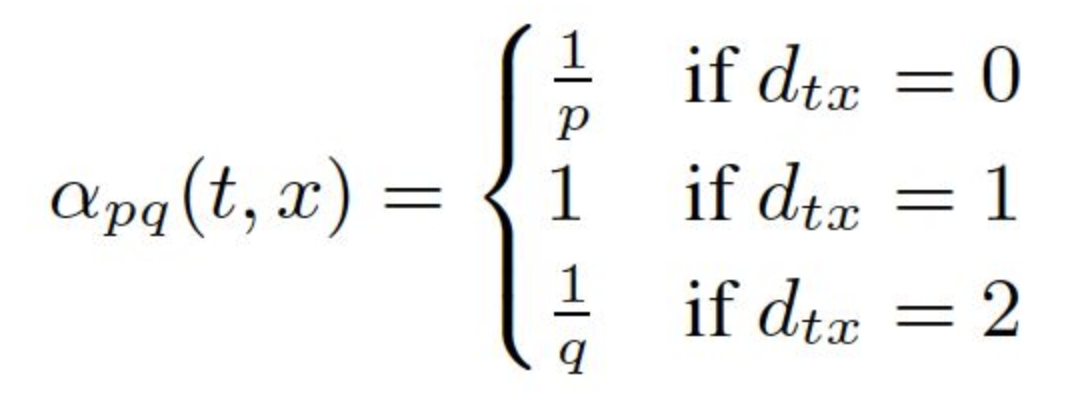
\includegraphics[width=.6\textwidth]{fig/Graph_Embedding_Node2Vec_Trans_Prob_3.png}
\end{figure}

其中,dtx指的是节点t到节点x的距离,参数p和q共同控制着随机游走的倾向性。参数p被称为返回参数(return parameter),p越小,随机游走回节点t的可能性越大,node2vec就更注重表达网络的同质性,参数q被称为进出参数(in-out parameter),q越小,则随机游走到远方节点的可能性越大,node2vec更注重表达网络的结构性,反之,当前节点更可能在附近节点游走。

node2vec这种灵活表达同质性和结构性的特点也得到了实验的证实。图6的上图就是node2vec更注重同质性的体现,可以看到距离相近的节点颜色更为接近,而图6下图则是结构特点相近的节点的颜色更为接近。
\begin{figure}[H]
    \centering
    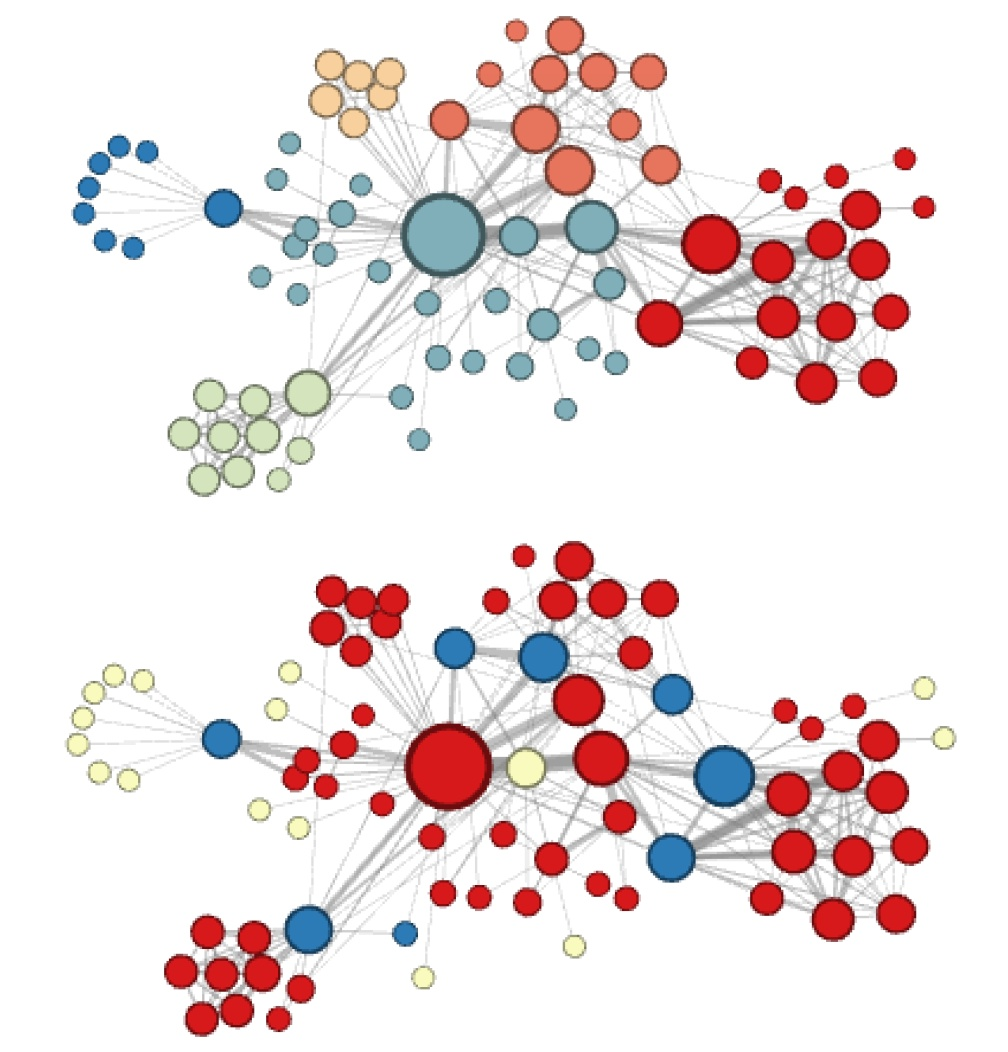
\includegraphics[width=.6\textwidth]{fig/Graph_Embedding_Node2Vec_Result_Example.jpg}
\end{figure}

node2vec所体现的网络的同质性和结构性在推荐系统中也是可以被很直观的解释的。同质性相同的物品很可能是同品类、同属性、或者经常被一同购买的物品,而结构性相同的物品则是各品类的爆款、各品类的最佳凑单商品等拥有类似趋势或者结构性属性的物品。毫无疑问,二者在推荐系统中都是非常重要的特征表达。由于node2vec的这种灵活性,以及发掘不同特征的能力,甚至可以把不同node2vec生成的embedding融合共同输入后续深度学习网络,以保留物品的不同特征信息。

\subsection{阿里的Graph Embedding方法EGES}
2018年阿里公布了其在淘宝应用的Embedding方法EGES(Enhanced Graph Embedding with Side Information),其基本思想是在DeepWalk生成的graph embedding基础上引入补充信息。

如果单纯使用用户行为生成的物品相关图,固然可以生成物品的embedding,但是如果遇到新加入的物品,或者没有过多互动信息的长尾物品,推荐系统将出现严重的冷启动问题。为了使“冷启动”的商品获得“合理”的初始Embedding,阿里团队通过引入了更多补充信息来丰富Embedding信息的来源,从而使没有历史行为记录的商品获得Embedding。

生成Graph embedding的第一步是生成物品关系图,通过用户行为序列可以生成物品相关图,利用相同属性、相同类别等信息,也可以通过这些相似性建立物品之间的边,从而生成基于内容的knowledge graph。而基于knowledge graph生成的物品向量可以被称为补充信息(side information)embedding向量,当然,根据补充信息类别的不同,可以有多个side information embedding向量。

那么如何融合一个物品的多个embedding向量,使之形成物品最后的embedding呢?最简单的方法是在深度神经网络中加入average pooling层将不同embedding平均起来,阿里在此基础上进行了加强,对每个embedding加上了权重,如图7所示,对每类特征对应的Embedding向量,分别赋予了权重a0,a1…an。图中的Hidden Representation层就是对不同Embedding进行加权平均操作的层,得到加权平均后的Embedding向量后,再直接输入softmax层,这样通过梯度反向传播,就可以求的每个embedding的权重ai(i=0…n)。
\begin{figure}[H]
    \centering
    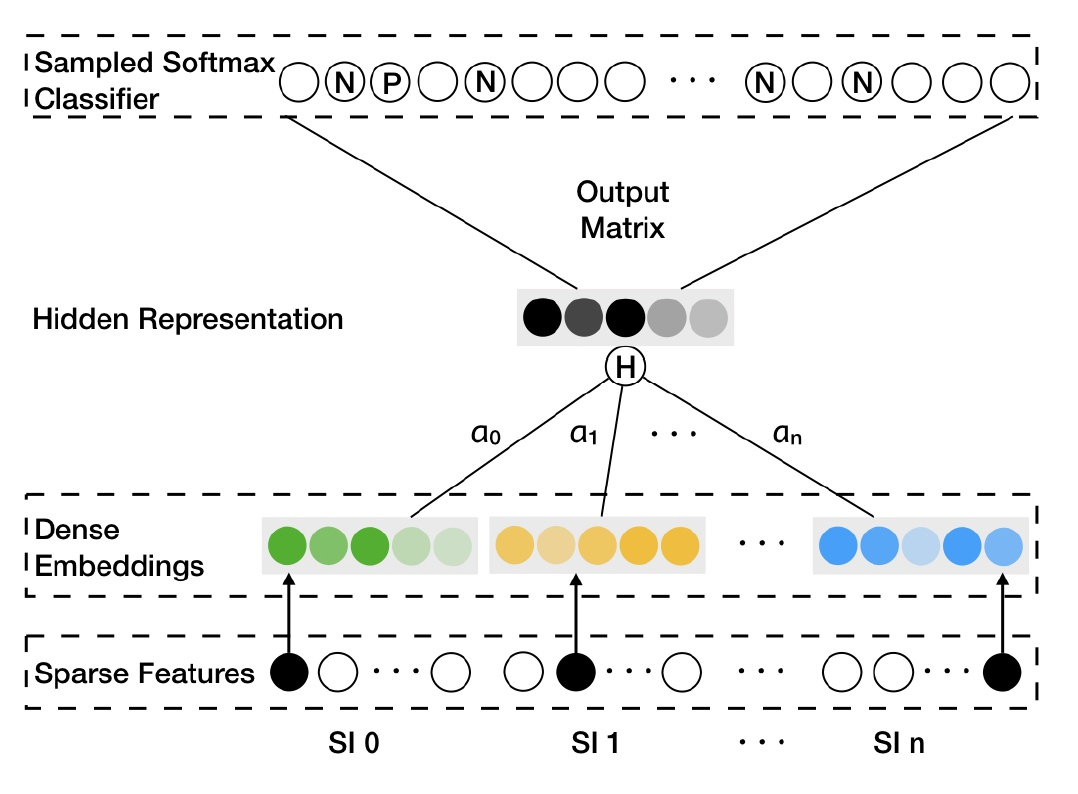
\includegraphics[width=.6\textwidth]{fig/Graph_Embedding_In_Ali.jpg}
\end{figure}

在实际的模型中,阿里采用了 $e^{a_j}$ 而不是aj作为相应embedding的权重,一是避免权重为0,二是因为$e^{a_j}$ 在梯度下降过程中有良好的数学性质。

阿里的EGES并没有过于复杂的理论创新,但给出一个工程性的结合多种Embedding的方法,降低了某类Embedding缺失造成的冷启动问题,是实用性极强的Embedding方法。

\part{Embedding 在工业场景的应用}
\section{Embedding 在 Airbnb 搜索排序中的应用
\cite{Embedding_In_Realtime_Search_In_Airbnb}\cite{How_Airbnb_Solve_Sparse_Problem_In_Embedding}}
论文名称: Real-time Personalization using Embeddings for Search Ranking at Airbnb 

Airbnb 作为全世界最大的短租网站,提供了一个连接房主(host)挂出的短租房(listing)和主要是以旅游为目的的租客(guest/user)的中介平台。这样一个中介平台的交互方式比较简单,guest 输入地点,价位,关键词等等,Airbnb 会给出 listing 的搜索推荐列表

容易想见,接下来guest和host之间的交互方式无非有这样几种:
\begin{itemize}
\setlength{\itemsep}{0pt}
\setlength{\parsep}{0pt}
\setlength{\parskip}{0pt}
    \item guest点击listing (click);
    \item guest预定lising (book);
    \item host有可能拒绝guest的预定请求 (reject);
\end{itemize}
\begin{figure}[H]
    \centering
    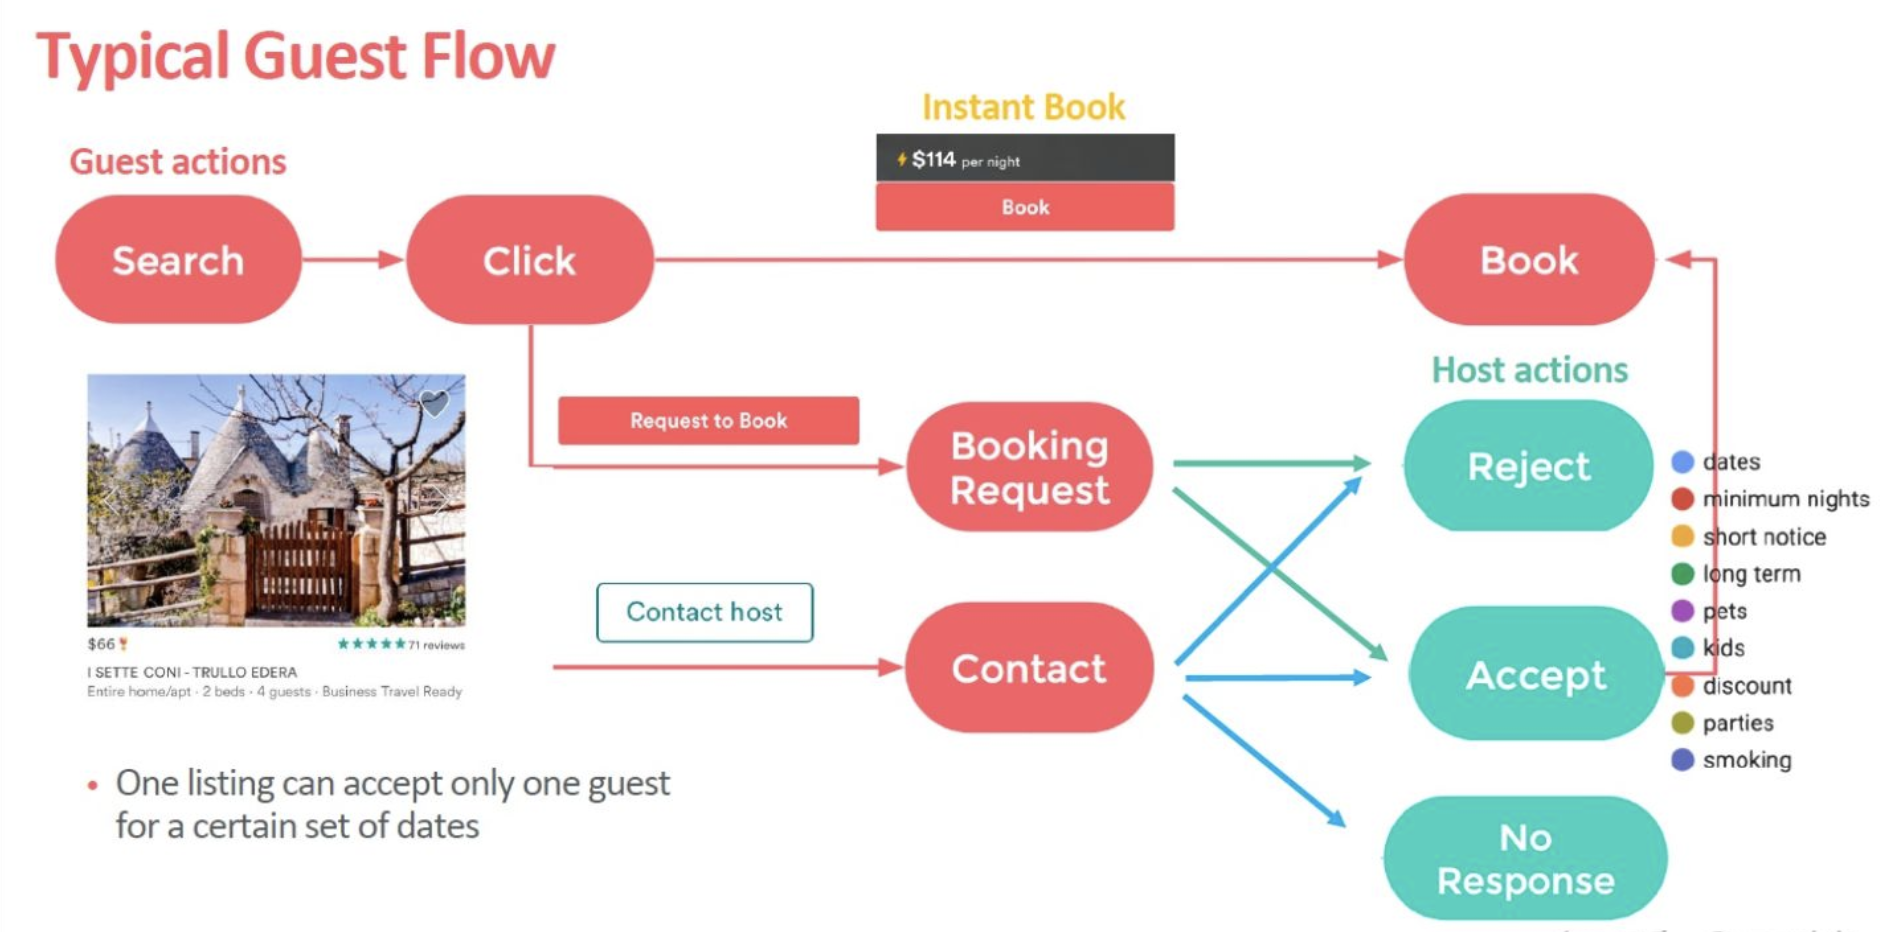
\includegraphics[width=1\textwidth]{fig/Airbnb_User_Interaction.png}
\end{figure}

基于这样的场景,利用几种交互方式产生的数据,Airbnb的search团队要构建一个real time的ranking model。\textbf{为了捕捉到用户short term以及long term的兴趣,Airbnb并没有把user history的clicked listing ids或者booked listing ids直接输入ranking model,而是先对user和listing进行了embedding,进而利用embedding的结果构建出诸多feature,作为ranking model的输入}。这篇文章的核心内容就是介绍如何\textbf{生成listing和user的embedding}。

具体到embedding上,文章通过两种方式生成了两种不同的embedding分别capture用户的short term和long term的兴趣。
\begin{itemize}
\setlength{\itemsep}{0pt}
\setlength{\parsep}{0pt}
\setlength{\parskip}{0pt}
    \item \textbf{通过click session数据生成listing的embedding},生成这个embedding的目的是为了\textcolor{red}{进行listing的相似推荐,以及对用户进行session内的实时个性化推荐};
    \item \textbf{通过booking session生成user-type和listing-type的embedding},目的是\textcolor{red}{捕捉不同user-type的long term喜好}。由于booking signal过于稀疏,Airbnb对同属性的user和listing进行了聚合,形成了user-type和listing-type这两个embedding的对象;
\end{itemize}

\subsection{对listing进行embedding的方法}
Airbnb采用了click session数据对listing进行embedding,其中\textbf{click session指的是一个用户在一次搜索过程中,点击的listing的序列}。这个序列需要满足两个条件,一个是只有停留时间超过30s的listing page才被算作序列中的一个数据点,二是如果用户超过30分钟没有动作,那么这个序列会断掉,不再是一个序列。

\begin{figure}[H]
    \centering
    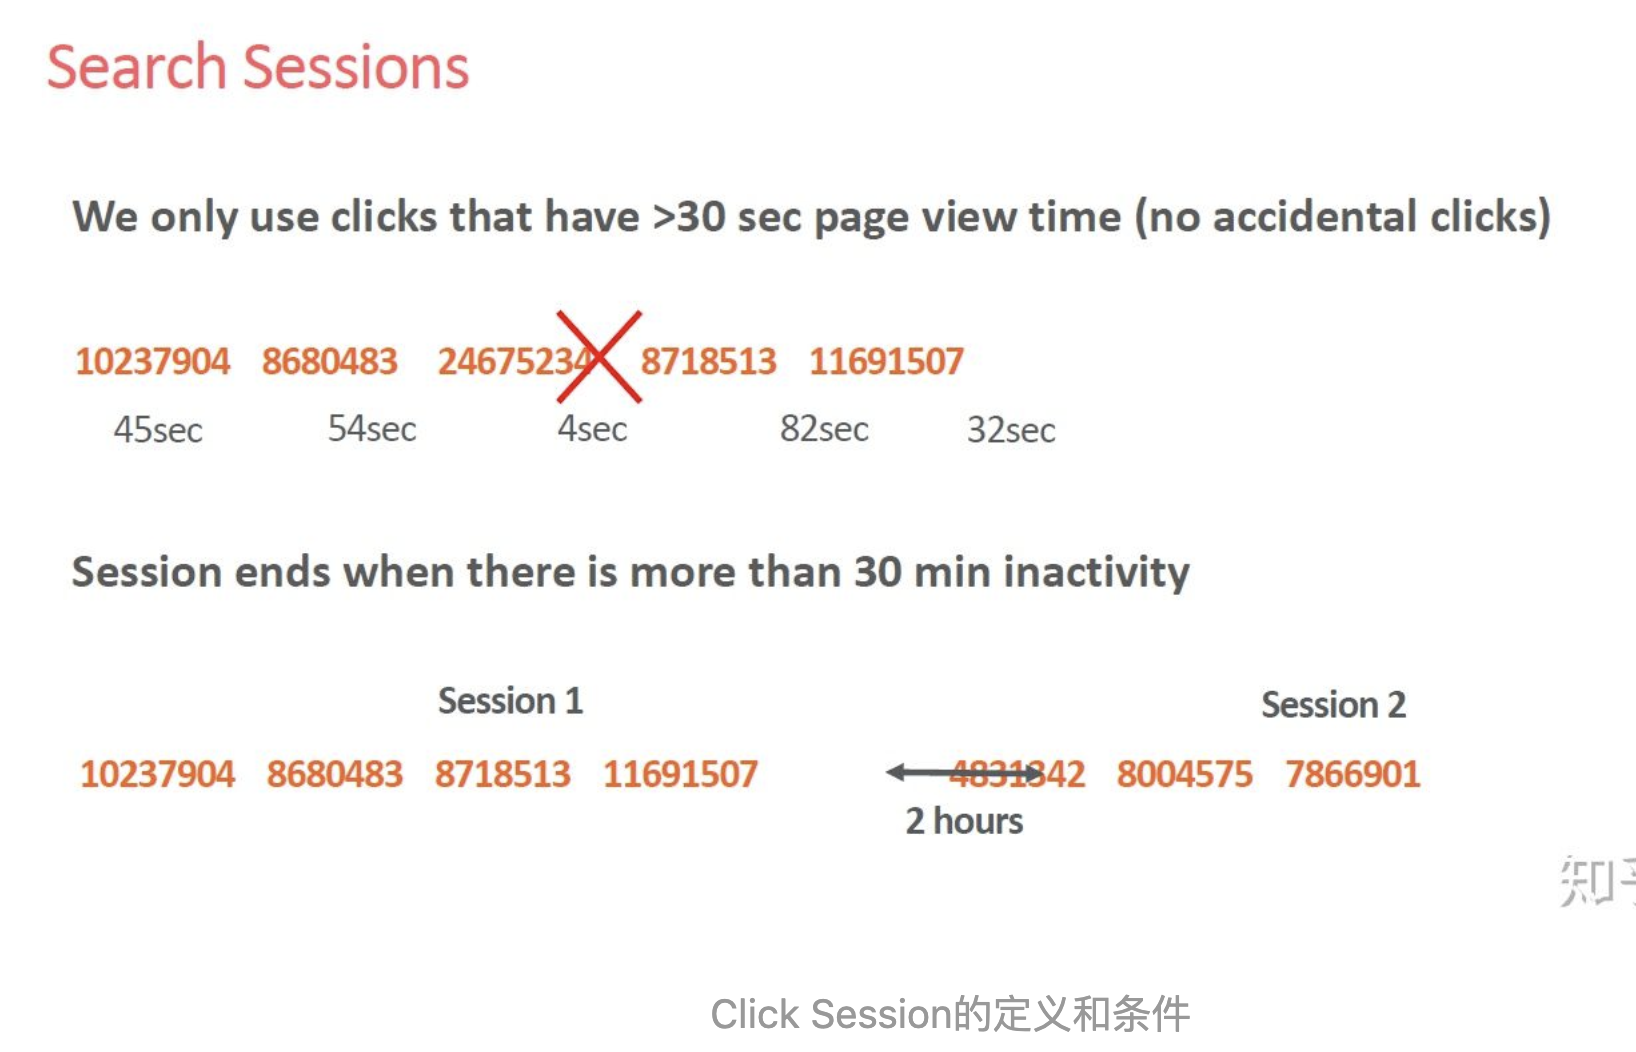
\includegraphics[width=1\textwidth]{fig/Airbnb_Click_Sessions.png}
\end{figure}

这么做的目的:一是清洗噪声点和负反馈信号,二是避免非相关序列的产生。

有了由clicked listings组成的sequence,就像我们在之前专栏文章中讲过的item2vec方法一样,我们可以把这个sequence当作一个“句子”样本,开始embedding的过程。Airbnb不出意外的选择了word2vec的skip-gram model作为embedding方法的框架。通过修改word2vec的objective使其靠近Airbnb的业务目标。
\begin{figure}[H]
    \centering
    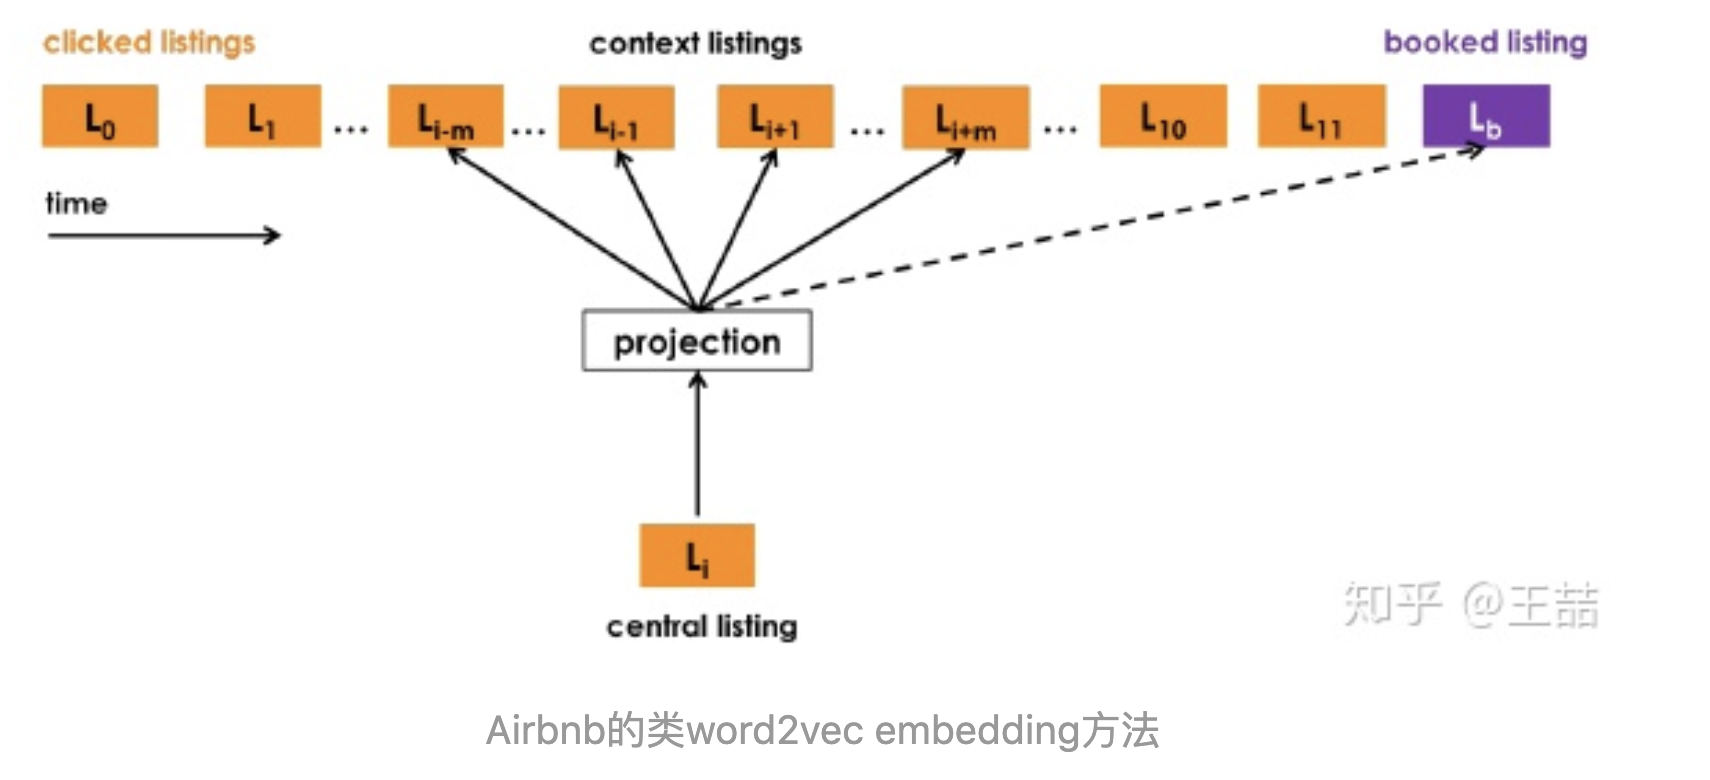
\includegraphics[width=1\textwidth]{fig/Airbnb_Word2Vec_Embedding_For_Session.png}
\end{figure}

这里直接列出word2vec的skip-gram model的objective如下:
$$
\arg\max_\theta \sum_{(w,c) \in D} \log{p(c|w)} = \sum_{(w,c) \in D}(\log{e^{v_c \cdot v_w}} - \log{\sum_{c'}e^{v_{c'} \cdot v_w}})
$$


在采用negative sampling的训练方式之后,objective转换成了如下形式:
$$
\arg\max_\theta \sum_{(w,c) \in D} \log{\sigma(v_c \cdot v_w)} +  \sum_{(w,c) \in D'}\log{\sigma(-v_c \cdot v_w)}
$$

其中 $\sigma$ 函数代表的就是我们经常见到的sigmoid函数,D是正样本集合,D'是负样本集合。我们再详细看一下上面word2vec这个objective function,其中前面的部分是正样本的形式,后面的部分是负样本的形式(仅仅多了一个负号)。

为什么原始的objective可以转换成上面的形式,其实并不是显然的,感兴趣的同学可以参考这篇文章, Negative-Sampling Word-Embedding Method。这里,我们就以word2vec的objective function为起点,开始下面的内容。

转移到Airbnb这个问题上,正样本很自然的取自click session sliding window里的两个listing,负样本则是在确定central listing后随机从语料库(这里就是listing的集合)中选取一个listing作为负样本。

因此,Airbnb初始的objective function几乎与word2vec的objective一模一样,形式如下:
\begin{figure}[H]
    \centering
    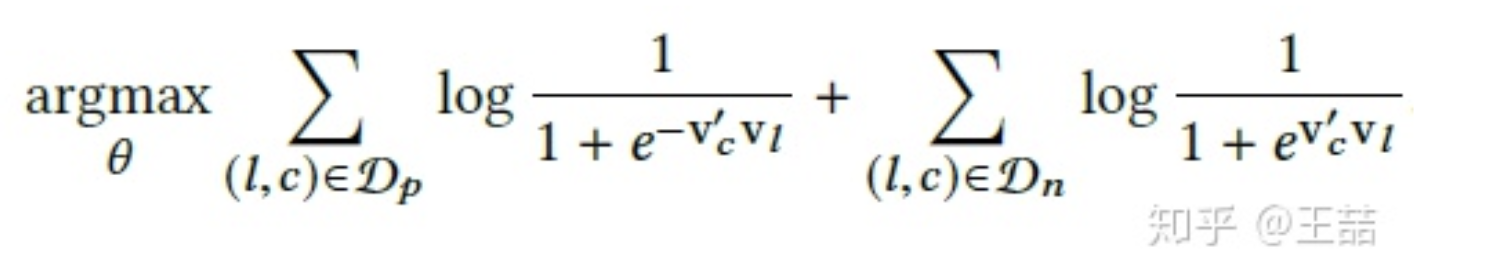
\includegraphics[width=1\textwidth]{fig/Airbnb_Click_Objetive.png}
\end{figure}


在原始word2vec embedding的基础上,针对其业务特点,Airbnb的工程师希望能够把booking的信息引入embedding。这样直观上可以使Airbnb的搜索列表和similar item列表中更倾向于推荐之前booking成功session中的listing。从这个motivation出发,Airbnb把click session分成两类,最终产生booking行为的叫booked session,没有的称做exploratory session。

因为每个booked session只有最后一个listing是booked listing,所以为了把这个booking行为引入objective,我们不管这个booked listing在不在word2vec的滑动窗口中,我们都会假设这个booked listing与滑动窗口的中心listing相关,所以相当于引入了一个global context到objective中,因此,objective就变成了下面的样子
\begin{figure}[H]
    \centering
    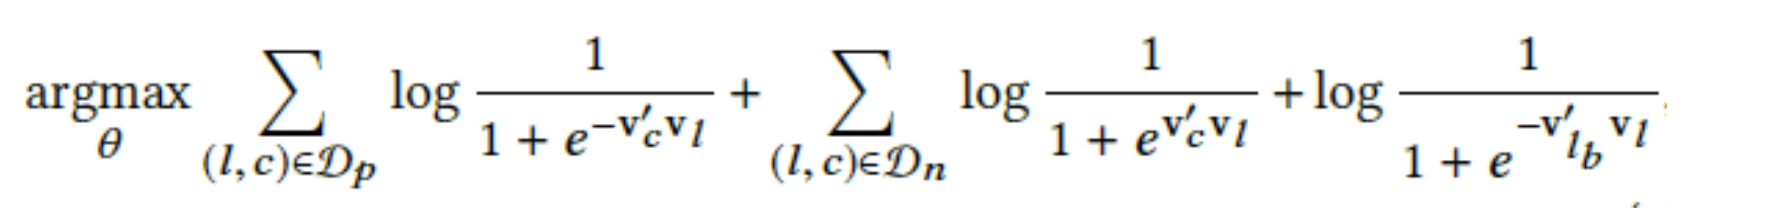
\includegraphics[width=1\textwidth]{fig/Airbnb_Click_Objetive2.png}
\end{figure}

其中最后一项的lb就是代表着booked listing,因为booking是一个正样本行为,这一项前也是有负号的。

需要注意的是最后一项前是没有sigma符号的,前面的sigma符号是因为滑动窗口中的中心listing与所有滑动窗口中的其他listing都相关,最后一项没有sigma符号直观理解是因为booked listing只有一个,所以central listing只与这一个listing有关。

但这里的objective的形式我仍让是有疑问的,因为这个objective写成这种形式应该仅代表了一个滑动窗口中的objective,并不是整体求解的objective。如果是整体的objective,理应是下面的形式:
\begin{figure}[H]
    \centering
    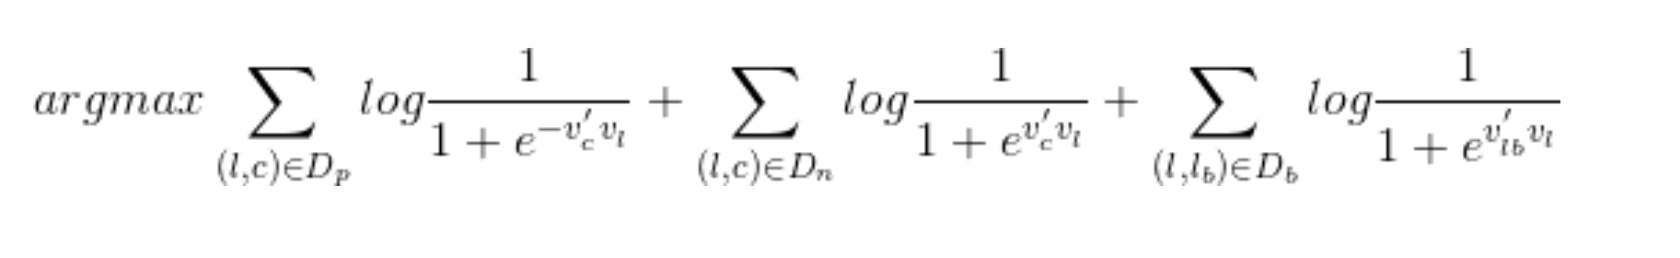
\includegraphics[width=1\textwidth]{fig/Airbnb_Click_Objetive3.png}
\end{figure}

其中Db代表了所有booked session中所有滑动窗口中central listing和booked listing的pair集合。

下面这一项就比较容易理解了,为了更好的发现同一市场(marketplace)内部listing的差异性,Airbnb加入了另一组negative sample,就是在central listing同一市场的listing集合中进行随机抽样,获得一组新的negative samples。同理,我们可以用跟之前negative sample同样的形式加入到objective中。
\begin{figure}[H]
    \centering
    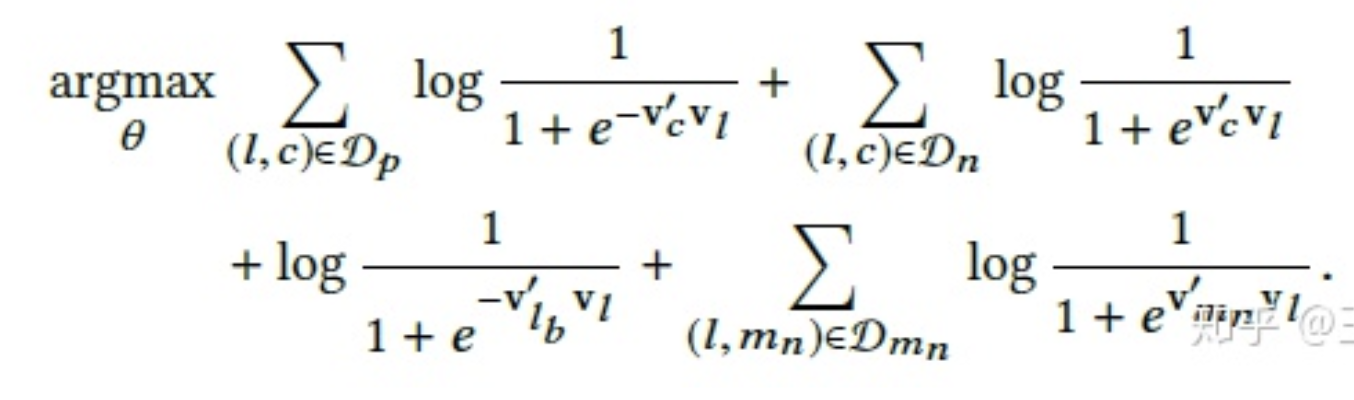
\includegraphics[width=1\textwidth]{fig/Airbnb_Click_Objetive4.png}
\end{figure}

其中Dmn就是新的同一地区的negative samples的集合。

至此,lisitng embedding的objective就定义完成了,embedding的训练过程就是word2vec negative sampling模型的标准训练过程,这里不再详述。

除此之外,文章多介绍了一下\textbf{cold start}的问题。简言之,\textbf{如果有new listing缺失embedding vector,就找附近的3个同样类型、相似价格的listing embedding进行平均得到},不失为一个实用的工程经验。

\subsection{对 booking 进行 embedding 的方法}
上面我们介绍了Airbnb为了捕捉用户的短期兴趣,使用用户的点击数据构建了listing(也可称为item,即一个短租屋)的 embedding,基于该embedding,可以很好的找出相似listing,但有所欠缺的是,该embedding并没有包含用户的长期兴趣信息。比如用户6个月前订了一个listing,其中包含了该用户对于房屋价格、房屋类型等属性的长期偏好,但由于之前的embedding只使用了session级别的点击数据,从而明显丢失了用户的长期兴趣信息。

为了捕捉用户的长期偏好,airbnb在这里使用了booking session序列。比如用户j在过去1年依次book过5个listing,那么其booking session就是$s_j = (l_{j1}, l_{j2}, l_{j3}, l_{j4}, l_{j5})$。既然有了booking session的集合,我们是否可以像之前对待click session一样拿直接应用w2v的方法得到embedding呢?答案是否定的,因为我们会遇到非常棘手的\textbf{数据稀疏}问题。

具体来讲booking session的数据稀疏问题表现在下面三点上:
\begin{itemize}
\setlength{\itemsep}{0pt}
\setlength{\parsep}{0pt}
\setlength{\parskip}{0pt}
    \item book行为的总体数量本身就远远小于click的行为,所以booking session集合的大小是远远小于click session的;
    \item 单一用户的book行为很少,大量用户在过去一年甚至只book过一个房源,这导致很多booking session sequence的长度为1
;
\end{itemize}

Airbnb如何解决如此严重的数据稀疏问题,训练出有意义的user embedding和listing embedding呢?
他们给出的答案是\textbf{基于某些属性规则做相似user和相似listing的聚合}。

举例来说,listing的属性如下表所示:
\begin{figure}[H]
    \centering
    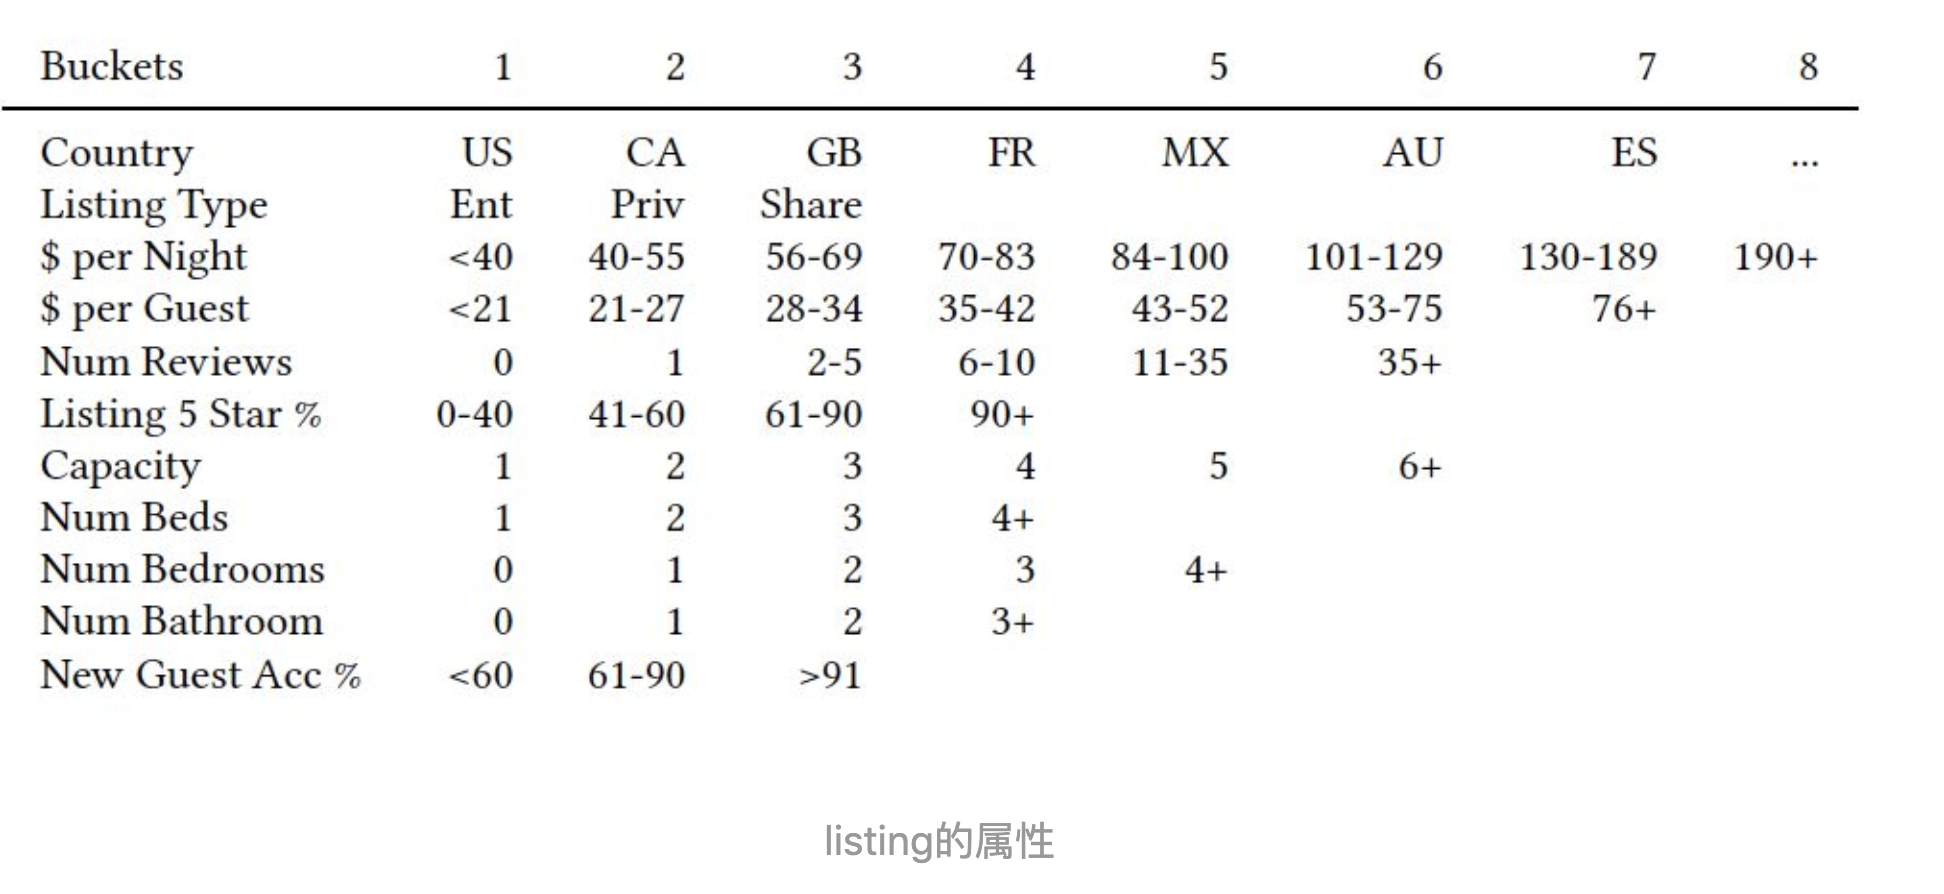
\includegraphics[width=1\textwidth]{fig/Airbnb_Booking_Listing_Attrs.png}
\end{figure}

那么我们就可以用属性名和bucket id组成一个属性标识,比如说某个listing的国家是US,类型(listing type)是Ent(bucket 1),每晚的价格(per night)是56-59美金(bucket3),那么就可以用US\_lt1\_pn3来表示该listing的listing\_type。

user\_type的定义同理,我们可以看一下airbnb用了什么用户属性,从下表中我们看到有device type,是否填了简介,有没有头像照片,之前定过的平均价位等等,可以看出都是一些非常基础和通用的属性,这对于我们来说也有借鉴意义,因为任何网络服务都可以很容易的找出这些属性。

\begin{figure}[H]
    \centering
    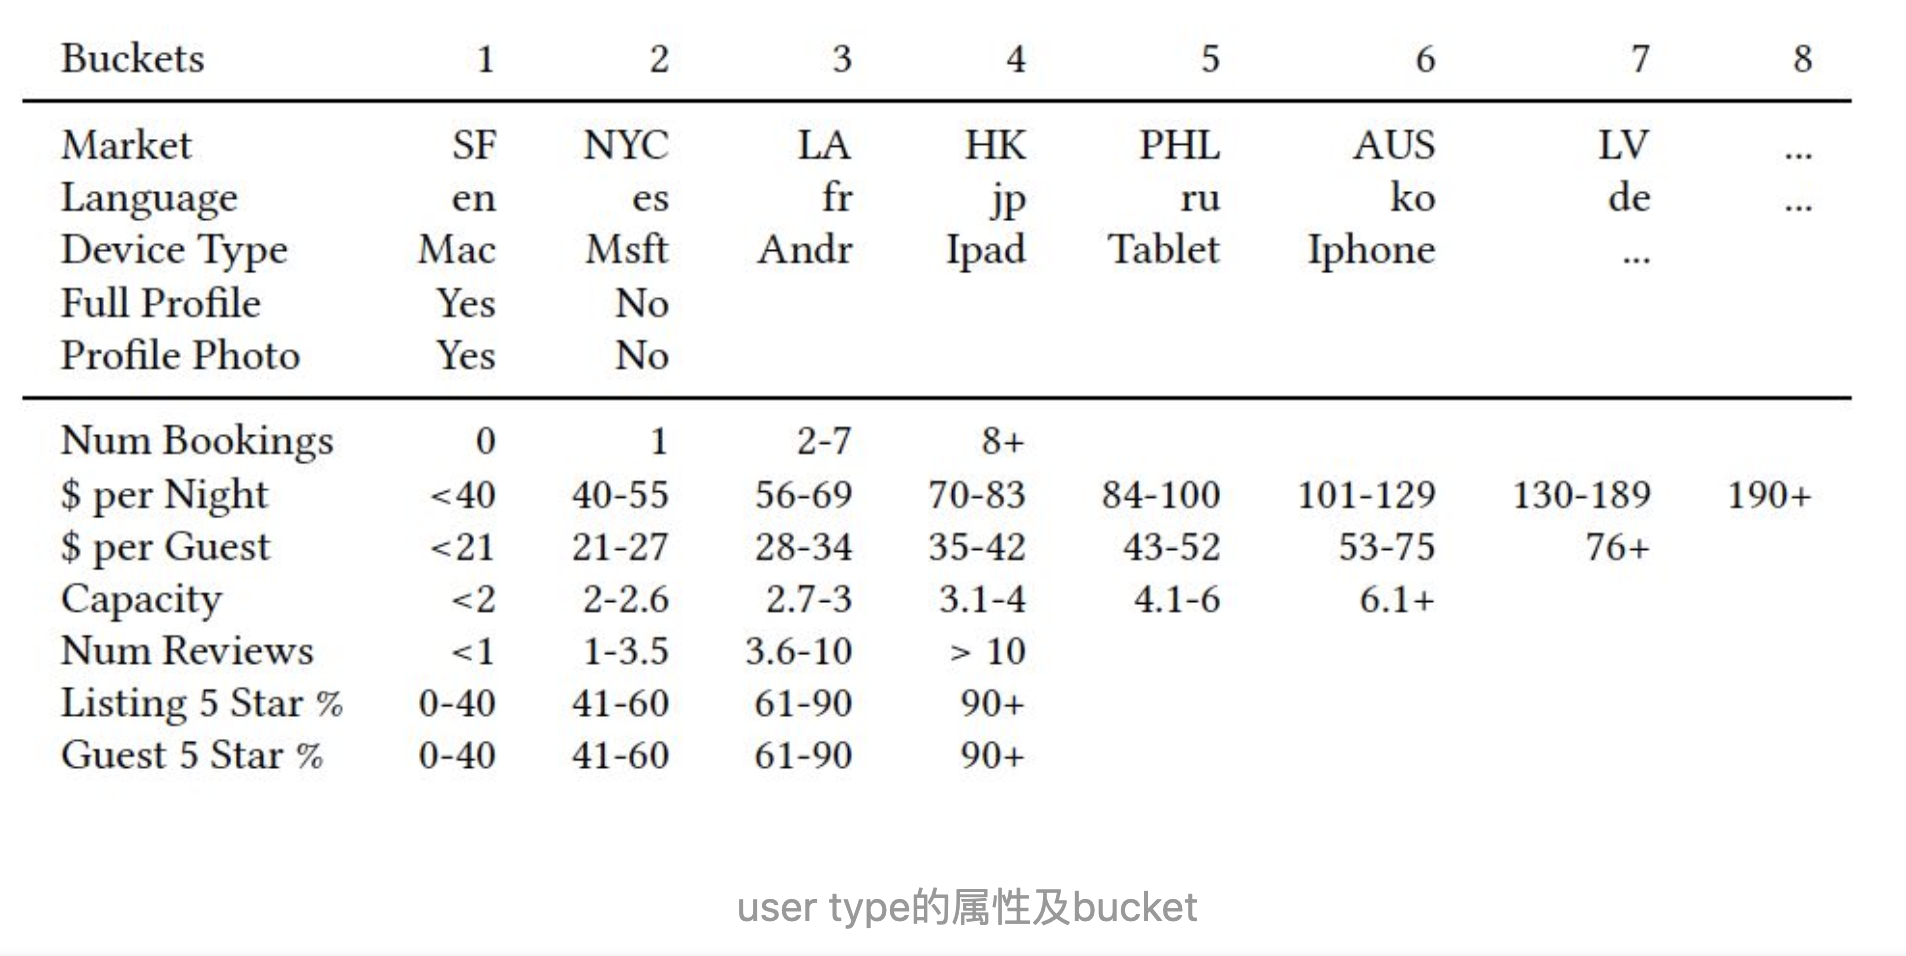
\includegraphics[width=1\textwidth]{fig/Airbnb_User_Type_And_Buckets.png}
\end{figure}

有了user type和listing type之后,一种直观的生成新的booking session sequence的方式是这样,\textbf{直接把user type当作原来的user id,生成一个由listing type组成的booking session}。这种方法能够解决数据稀疏性的问题,却无法直接得到user type embedding。为了让user type embedding和listing type embedding在同一个vector space中生成,airbnb采用了一种比较“反直觉”的方式。

针对某一user id按时间排序的booking session,$(l_1, l_2, \cdots, l_M)$,我们用(user\_type, listing\_type)组成的元组替换掉原来的listing item,因此sequence变成了$((u_{type1}, l_{type1}), (u_{type2}, l_{type2}), \cdots, (u_{typeM}, l_{typeM}))$ ,这里 $l_{type1}$ 指的就是listing l1对应的listing type, $u_{type1}$ 指的是该user在book listing l1时的user type,由于某一user的user\_type会随着时间变化,所以 $u_{type1}, u_{type2}$不一定相同。

有了该sequence的定义,下面的问题就是如何训练embedding使得user type和listing type在一个空间内了。训练所用的objective完全沿用了上一篇文章的objective的形式,但由于我们用一个(user type,listing type)的元组替换掉了原来的listing,如何确定central item就成为了一个核心问题。针对该问题,文章的原话是这么说的。

\begin{framed}
instead of listing l , the center item that needs to be updated is either user\_type (ut) or listing\_type (lt) depending on which one is caught in the sliding window.
\end{framed}

这个表述很有意思但也比较模糊,就是说在通过sliding window的形式计算objective的时候,central item可以是user type 也可以是listing type,这取决于我们在sliding window中“抓住”了哪个。

什么叫“抓住”?如何“抓住”,文章没有给出精确的定义,非常欢迎大家作出自己的解读。这里我先给出我的猜测。

因为文章之后列出了central item分别是user type和item type时的objective如下

\begin{figure}[H]
    \centering
    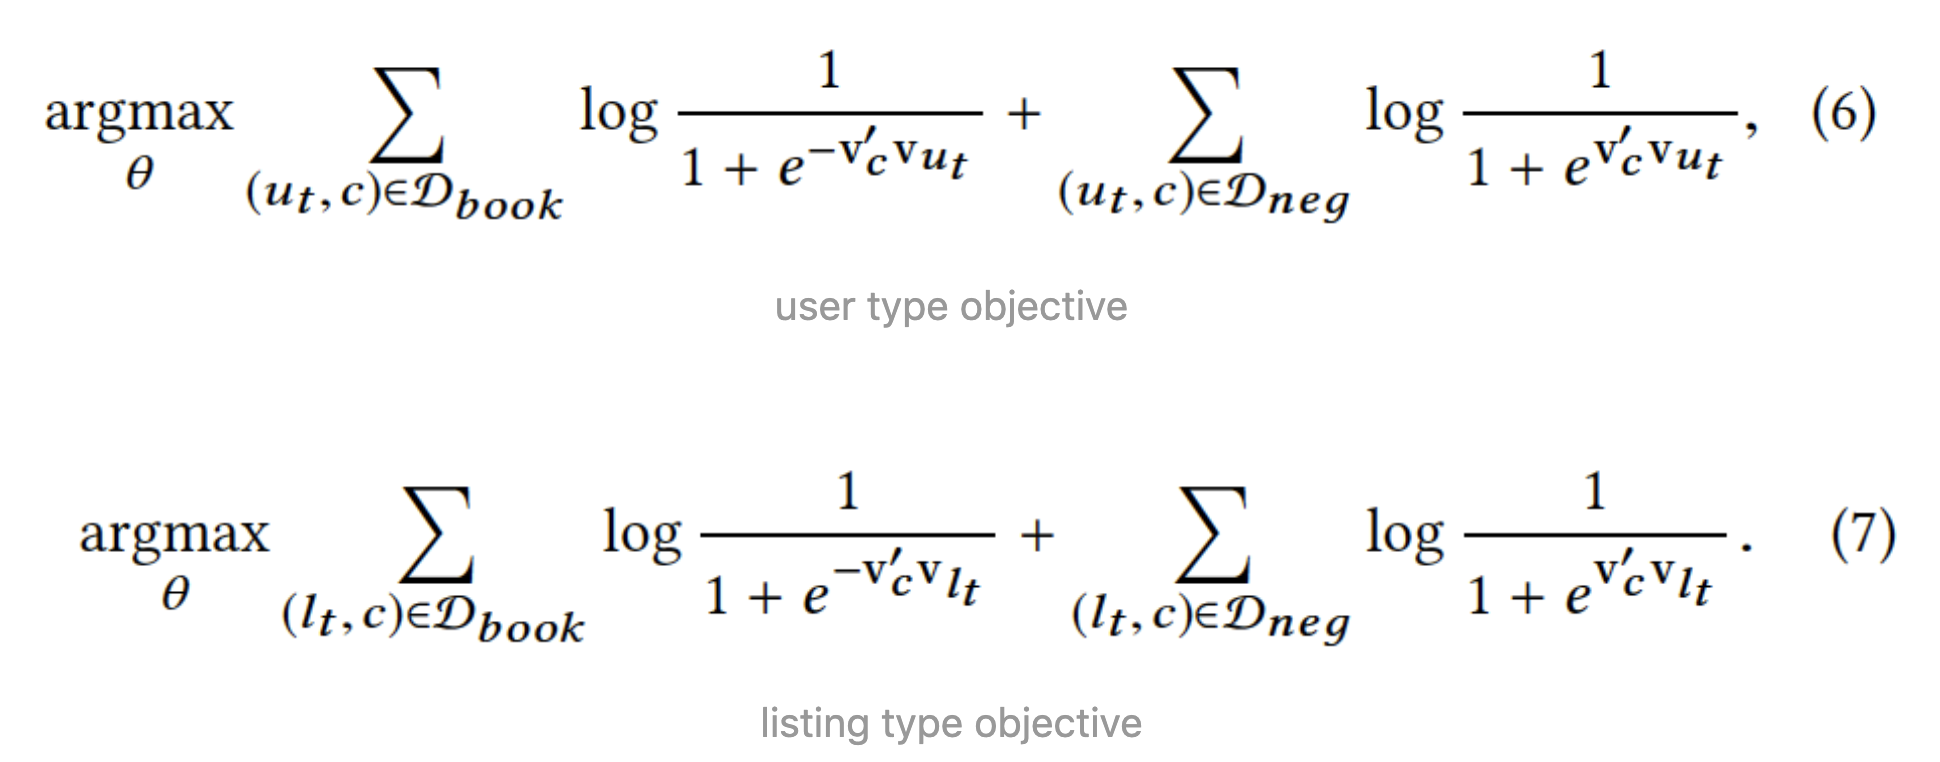
\includegraphics[width=1\textwidth]{fig/Airbnb_Click_Objetive5.png}
\end{figure}

其中$D_{book}$是central item附近的user type和item type的集合。如果这样的话,这两个objective是完全一样的。

所以我推测airbnb应该是把所有元组扁平化了一下,把user type和item type当作完全相同的item去训练embedding了,如果是这样的话二者当然是在一个vector space中。虽然整个过程就很tricky,但也不失为一个好的工程解决办法。

这里我再次征求大家对于这个问题的见解,非常欢迎你的看法。

接下来为了引入“房主拒绝”(reject)这个action,airbnb又在objective中加入了reject这样一个negative signal,方法与上一篇文章中加入negative signal的方法相同,在此不再赘述。

其实除了计算user embedding外,airbnb在分享的slides中提到他们还直接把query embedding了,从最后的搜索效果来看,query embedding跟listing embedding也是处于一个vector space,大家可以从下图中看出embedding方法的神奇。
\begin{figure}[H]
    \centering
    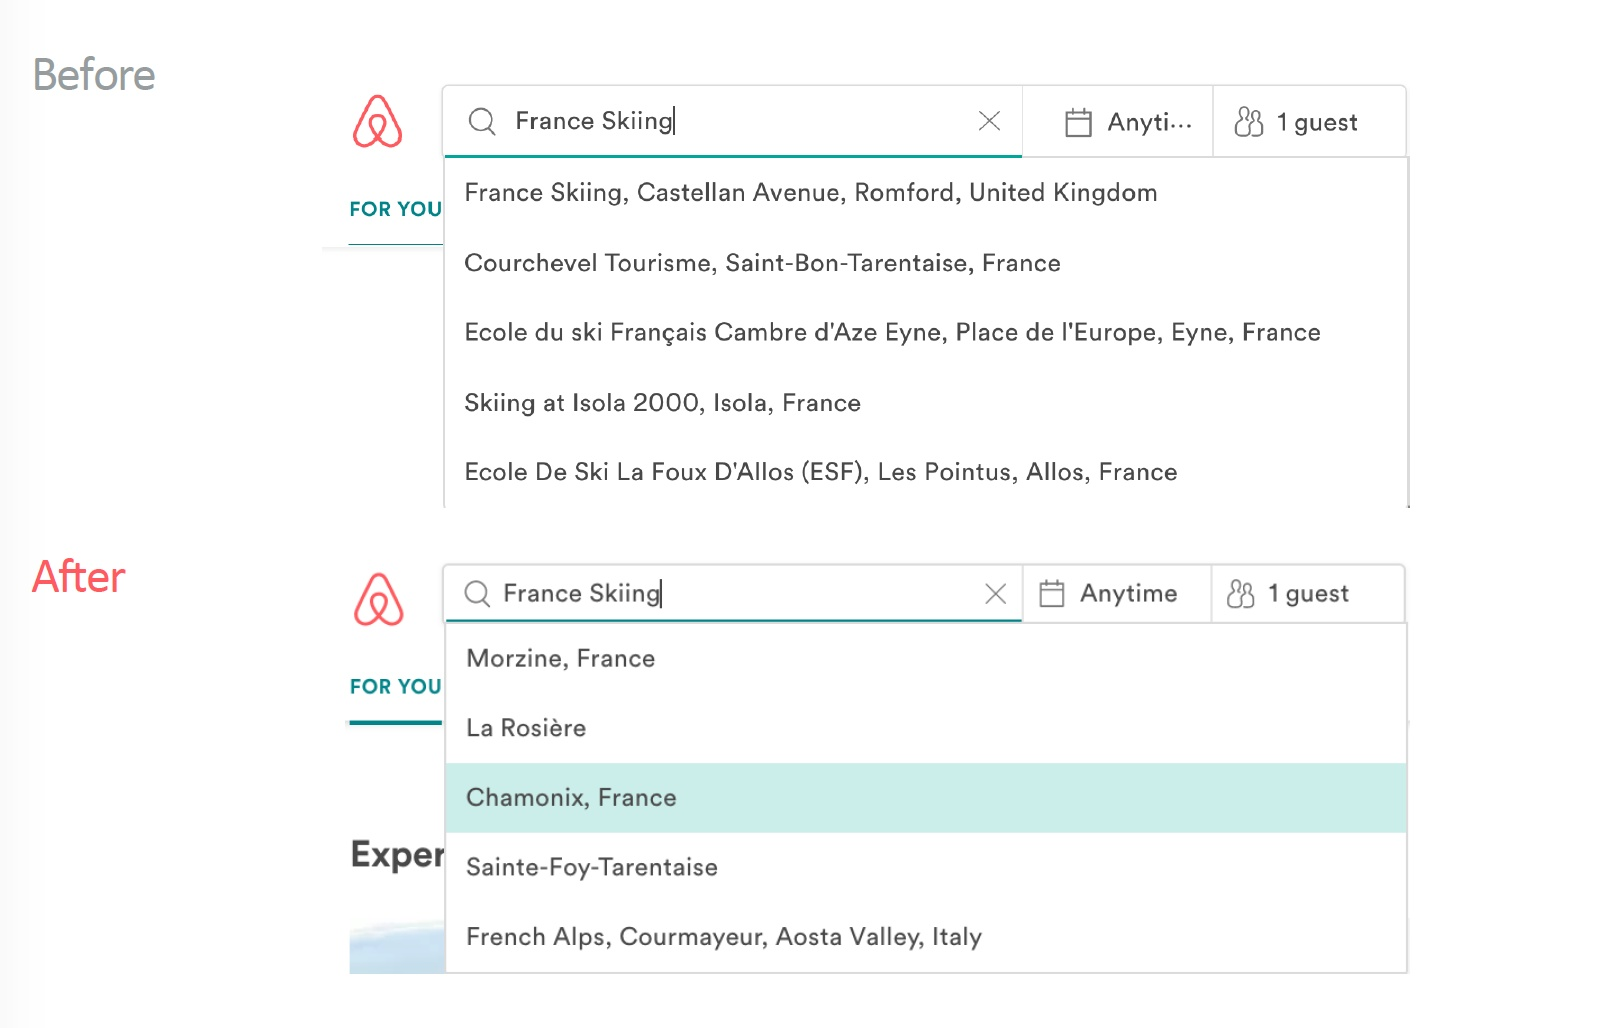
\includegraphics[width=1\textwidth]{fig/Airbnb_Search_Embedding.jpg}
\end{figure}

可以看到,在引入embedding之前,搜索结果只能是文本上的关键词搜索,引入embedding之后,搜索结果甚至能够捕捉到搜索词的语义信息。比如输入France Skiing,虽然结果中没有一个listing带有Skiing这个关键词,但这个结果无一例外都是法国的滑雪胜地,这无疑是更接近用户动机的结果。

在这篇Slides中Airbnb并没有具体介绍是如何生成query embedding,大家可以思考一下query embedding的具体生成过程。

到此我介绍完了airbnb所有的embedding方法,这里我要强调的是,airbnb并没有直接把embedding similarity直接得到搜索结果,而是基于embedding得到不同的user-listing pair feature,然后输入搜索排序模型,得到最终的排序结果。下面我们来看一看airbnb的搜索排序模型和feature。

\textbf{airbnb采用的搜索排序模型是一个pairwise的支持Lambda Rank的GBDT模型}。该模型已经由airbnb的工程师开源,感兴趣的同学可以去学习一下(github地址:https://github.com/yarny/gbdt)。

我们关注的重点回到特征工程上来,airbnb基于embedding生成了哪些feature呢?这些feature又是如何驱动搜索结果的“实时”个性化呢?

下面列出了基于embedding的所有feature。
\begin{figure}[H]
    \centering
    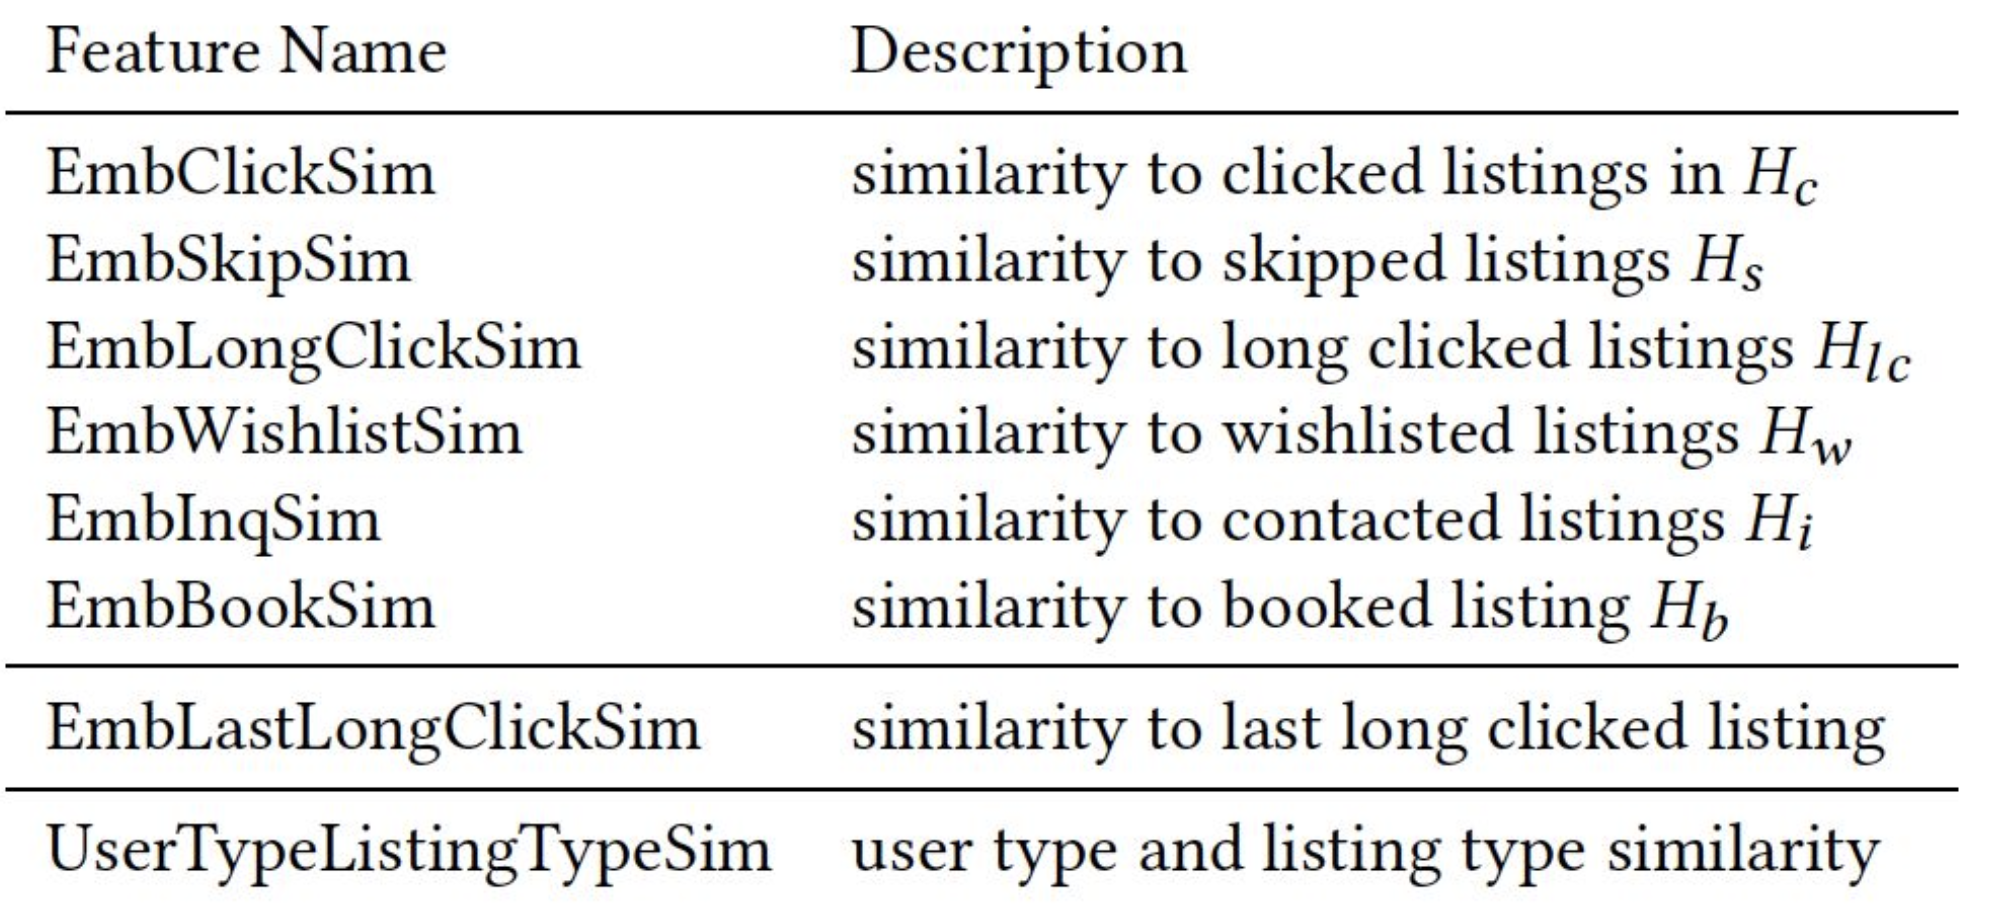
\includegraphics[width=1\textwidth]{fig/Airbnb_Embedding_Features.png}
\end{figure}

我们可以很清楚的看到,最后一个feature UserTypeListingTypeSim指的是 user type和listing type的similarity,该feature使用了我们这篇文章介绍的包含用户长期兴趣的embedding,除此之外的其他feature都是基于上篇文章介绍的listing embedding。比如EmbClickSim指的是candidate listing与用户最近点击过的listing的相似度。

这里我想我们可以回答这个问题了,为什么airbnb在文章题目中强调是real time personalization?\textbf{原因就是由于在这些embedding相关的feature中,我们加入了“最近点击listing的相似度”,“最后点击listing的相似度”这类特征,由于这类特征的存在,用户在点击浏览的过程中就可以得到实时的反馈,搜索结果也是实时地根据用户的点击行为而改变,所以这无疑是一个real time个性化系统}。


\section{扩展阅读}
Embedding从入门到专家必读的十篇论文:\url{https://zhuanlan.zhihu.com/p/58805184}

%\printbibliography
\bibliography{../ref}
\bibliographystyle{IEEEtran}
\end{document}